\documentclass[letterpaper,11pt,nointlimits,reqno,draft]{amsart}

% Avoid "Too many math alphabets used in version normal" issue
\newcommand\hmmax{0}
\newcommand\bmmax{0}

% Load the color package first to avoid option clashes
\usepackage[usenames,dvipsnames,svgnames,table]{xcolor}

% Packages
\usepackage{accents}
\usepackage{algorithm}
\usepackage{algorithmic}
\usepackage{amsfonts}
\usepackage{amsmath}
\usepackage{amssymb}
\usepackage{bm}
\usepackage{enumerate}
\usepackage{fancyhdr}
\usepackage{floatpag}
\usepackage{fullpage}
\usepackage{ifthen}
\usepackage{lastpage}
\usepackage{latexsym}
\usepackage{mathrsfs}
\usepackage{mathtools}
\usepackage[numbers,sort&compress]{natbib}
\usepackage{parskip}
\usepackage{pstricks}
\usepackage{rotating}
\usepackage{setspace}
%\usepackage{txfonts}
\usepackage{units}
\usepackage{varioref}
\usepackage{wrapfig}
\usepackage{yhmath}

\usepackage[obeyDraft,textsize=scriptsize]{todonotes}

% Hyperref package must be last otherwise the contents are jumbled
% hypertexnames disabled to fix links pointing to incorrect locations
\usepackage[colorlinks=true,
            linkcolor=blue,
            urlcolor=blue,
            citecolor=blue,
            final,
            hypertexnames=false]{hyperref}

% In conjunction with -shell-escape, automatically convert EPS to PDF
\usepackage{epstopdf}
\epstopdfsetup{outdir=./,suffix=-generated,update,verbose}
\epstopdfDeclareGraphicsRule{.eps}{pdf}{.pdf}{%
    epstopdf --outfile=\OutputFile \space `kpsewhich \space "\SourceFile"`
}

% Fix Todonotes wrongly placed in the margin
\setlength{\marginparwidth}{2cm}

% Environment sidewaysfigure from rotating plays poorly with amsart class
% Fix per http://www.latex-community.org/forum/viewtopic.php?f=4&t=1742
\setlength\rotFPtop{0pt plus 1fil}

\mathtoolsset{showonlyrefs,showmanualtags}
%%% \allowdisplaybreaks[1] % Allow grouped equations to be split across pages

% Line Spacing
\singlespacing

% Increase table of contents depth
\setcounter{tocdepth}{4}

% Simplify headings on floating pages
\floatpagestyle{plain}
\rotfloatpagestyle{empty}

% Document-specific commands
\newcommand{\ii}{\ensuremath{\mathrm{i}}}
\newcommand{\trans}[1]{{#1}^{\ensuremath{\mathsf{T}}}}
\newcommand{\Knudsen}[1][]{\ensuremath{\mbox{Kn}_{#1}}}
\newcommand{\Mach}[1][]{\ensuremath{\mbox{Ma}_{#1}}}
\newcommand{\Reynolds}[1][]{\ensuremath{\mbox{Re}_{#1}}}
\newcommand{\Prandtl}[1][]{\ensuremath{\mbox{Pr}_{#1}}}
\newcommand{\reference}[1]{\ensuremath{\left\{#1\right\}_{0}}}
\newcommand{\lessreference}[1]
  {\ensuremath{\left({#1}-\reference{#1}\right)}}
\newcommand{\symmetricpart}[1]
  {\ensuremath{\operatorname{sym}\left(#1\right)}}
\DeclareMathOperator{\trace}{tr}
\newcommand{\Ssd}{\ensuremath{\mathcal{S}}} % source term due to slow derivative

% commands I like
\newcommand{\mbb}[1]{\mathbb{#1}}
\newcommand{\mbf}[1]{\mathbf{#1}}
\newcommand{\sbf}[1]{\boldsymbol{#1}}
\newcommand{\mcal}[1]{\mathcal{#1}}
\newcommand{\mfk}[1]{\mathfrak{#1}}
\newcommand{\pp}[2]{\frac{\partial #1}{\partial #2}}

\begin{document}

\title{Suzerain reacting flow model document}
\author{The PECOS Turbulence Group}
\date{\today}
\thanks{The Center for Predictive Engineering and Computational Sciences,
        The University of Texas at Austin}

\maketitle
\renewcommand{\contentsname}{} % No idea why "Contents" appears in wrong location
% From http://www.latex-community.org/forum/viewtopic.php?f=47&t=10536
\setcounter{tocdepth}{3}
\let\oldtocsection=\tocsection
\let\oldtocsubsection=\tocsubsection
\let\oldtocsubsubsection=\tocsubsubsection
\renewcommand{\tocsection}[2]{\hspace{0em}\oldtocsection{#1}{#2}}
\renewcommand{\tocsubsection}[2]{\hspace{1em}\oldtocsubsection{#1}{#2}}
\renewcommand{\tocsubsubsection}[2]{\hspace{2em}\oldtocsubsubsection{#1}{#2}}
\tableofcontents
\newpage

\section{Governing Equations}
This section details the equations that are to be discretized and
solved to simulate reacting flow in Suzerain.

\subsection{Conservation laws}
This section details the relevant conservation laws for chemically
  reacting flows.  Following~\cite{Anderson_hypersonics,
  Kirk_2009_FINS_model_doc,
  Topalian_2011_temporal_slow_growth_reacting}, the conservation of
  mass, momentum, and total energy for a compressible fluid composed
  of $N_s$ constitutive components may be written as
%
\begin{align*}
  \pp{\rho_{\alpha}}{t} & + \pp{}{x_j} (\rho_{\alpha} u_j + \rho_{\alpha} v_{\alpha, j}) = \dot{\omega}_{\alpha}, \\
  \pp{\rho}{t} & + \pp{}{x_j} (\rho u_j) = 0, \\
  \pp{\rho u_i}{t} & + \pp{}{x_j} (\rho u_j u_i + p \delta_{ji} - \tau_{ji}) = 0, \\
  \pp{\rho E}{t} & + \pp{}{x_j} \left(\rho u_j H + \sum_{\alpha=1}^{N_s} \rho_{\alpha} v_{\alpha, j} h_{\alpha}  - \tau_{ji} u_i + q_j \right) = 0,\\
\end{align*}
% 
where $\rho_{\alpha}$ is the density of species $\alpha$, $\rho=\sum_{\alpha} \rho_{\alpha}$
is the mixture density, $u_i$ is the mixture velocity in the $i$th
direction, $v_{\alpha, i}$ is the diffusion velocity of species $\alpha$ in the
$i$th direction, $E$ is the total energy per unit mass, $p$ is the
pressure, $H$ is the total enthalpy per unit mass, $\tau_{ji}$ is the
viscous stress tensor, and $q_j$ is the heat flux vector.  Note that
Roman indices ($i$, $j$) indicate spatial directions.  For these,
repeated indices imply summation.  Greek indices ($\alpha$) indicate
species, and repeated Greek indices do not imply summation.

Further note that there are more governing equations here than
unknowns.  This is resolved by the consistency between the
conservation of mass equation and the species conservation equations.
However, we must choose what set of equations to model and discretize.
Here, we choose to include the conservation of mass equation and $N_s
-1$ species conservation equations.  Further, the state variables will
be $\rho$, $\rho_{\alpha}$ for $\alpha \in 2, \ldots, N_s$, $\rho u_i$
for $i = 1, 2, 3$, and $\rho E$.  Thus, we have $N_s + 4$ state
variables, and, by convention, species $\alpha = 1$ is the diluter
(i.e., the species that is not explicitly tracked).

\subsection{Constitutive relations and other assumptions}
\label{sec:constitutive}

\subsubsection{Mass Diffusion}
Species diffusion is modeled using Fick's law.
Specifically, Fick's law is given by
%
\begin{equation*}
\rho_{\alpha} v_{\alpha, i} = - \rho \mcal{D}_{\alpha} \pp{c_{\alpha}}{x_i},
\end{equation*}
% 
where $\mcal{D}_{\alpha}$ is the mass diffusivity for species $\alpha$
and $c_{\alpha}$ is the mass fraction $\rho_{\alpha} / \rho$.
Suzerain uses a constant Lewis number model to compute the species
diffusivities:
%
\begin{equation*}
\mcal{D}_{\alpha} = \frac{Le \kappa}{\rho C_{p,\mathrm{mix}}},
\end{equation*}
%
where $Le$ is the Lewis number, $\kappa$ is the mixture thermal
conductivity, and $C_{p,\mathrm{mix}}$ is the mixture specific heat at
constant pressure.  

Note that, since $\mcal{D}_{\alpha}$ is the same for all $\alpha$ in
the mixture, the constant $Le$ model automatically satisfies
conservation of mass.

However, for complex models, the $\mcal{D}_{\alpha}$ values are in
general different for each $\alpha$.  In this case, the Fickian model
is not guaranteed to satisfy mass conservation.  That is,
%
\begin{equation*}
\sum_{\alpha = 1}^{N_s} \rho_{\alpha} v_{\alpha, i} = - \rho \sum_{\alpha = 1}^{N_s} \mcal{D}_{\alpha} \pp{c_{\alpha}}{x_i} \neq 0,
\end{equation*}
% 
leading to an extra term in the implied conservation of mass
equation.

To alleviate this problem, Ramshaw~\cite{?} devised the self-consistent
effective binary diffusion model.  In this model, each flux is
corrected as follows:
%
\begin{equation*}
\rho_{\alpha} v_{\alpha, i} = - \rho \mcal{D}_{\alpha} \pp{c_{\alpha}}{x_i} + c_{\alpha} \sum_{\beta = 1}^{N_s} \rho \mcal{D}_{\beta} \pp{c_{\beta}}{x_i}.
\end{equation*}
% 
Since $\sum_{\alpha} c_{\alpha} = 1$, this form clearly gives
$\sum_{\alpha} \rho_{\alpha} v_{\alpha,i} = 0$.

\subsubsection{Chemical Reactions}
The source terms $\dot{\omega}_{\alpha}$ in the species equations
appear due to chemical reactions.  At a given point in space and time,
these sources depend only on the state at that point in space and
time.  These terms will be evaluated from reaction mechanisms and
reaction rate models implemented in Antioch~\cite{?}.  The details of
these models will not be discussed further here.

\subsubsection{Viscous Stress}
The viscous stress is given by
%
\begin{equation*}
\tau_{ij} =  2 \mu \left[ \frac{1}{2} \left(\pp{u_i}{x_j} + \pp{u_j}{x_i} \right) - \frac{1}{3} \pp{u_k}{x_k} \delta_{ij} \right].
\end{equation*}
% 
Velocity derivatives are easily computed from the state derivatives,
and the viscosity $\mu$ is computed via a call to Antioch.

\subsubsection{Heat Flux}
The heat flux is given by
%
\begin{equation*}
q_j = - \kappa \pp{T}{x_j}.
\end{equation*}
% 
The temperature gradient is not easy to compute from derivatives of
state because an explicit functional form for the temperature given
the state is not available.  Thus, we will proceed by computing the
temperature field in physical space, transforming back to wave space,
differentiating, and transforming to physical space again.

The thermal conductivity is computed via a call to Antioch.

\subsubsection{Pressure and Temperature}
The mixture pressure is a sum of the species partial pressures:
%
\begin{equation*}
p = \sum_{\alpha = 1}^{N_s} p_{\alpha}.
\end{equation*}
%
Each partial pressure is computed from the ideal gas law,
%
\begin{equation*}
p_{\alpha} = \rho_{\alpha} R_{\alpha} T,
\end{equation*}
% 
where $R_{\alpha}$ is the gas constant for the species $\alpha$.  Thus,
%
\begin{equation*}
p = \rho R_{\mathrm{mix}} T,
\end{equation*}
% 
where $R_{\mathrm{mix}} = \sum_{s=1}^{N_s} c_s R_s$.  

Both $R_{\mathrm{mix}}$ and $T$ are obtained via calls to Antioch.

\subsubsection{Species Enthalpies}
Species enthalpies are determined using Antioch.


\subsection{Slow growth models}
\label{sec:slowgrowthmodels}
\todo{Document slow growth.  This will mainly be reference to Topalian's model docs.}








\section{Discretization}
This section describes the discretization of the conservation laws
described in \S\ref{sec:gov_eq}.  It draws heavily from the model
document for the perfect gas case~\cite{?} where appropriate.

\subsection{Spatial discretization}
For generality, write the continuous system of interest as
%
\begin{equation*}
\pp{u}{t} = \mathscr{L}u + \mathscr{N}\!\left(u\right) \quad \mathrm{for} \,\, (x,y,z) \in \Omega,
\end{equation*}
% 
where $u$ denotes the full state vector---i.e., $u = [\rho_{\alpha},
  \rho, \rho u_i, \rho E]^T$ for the reacting flow equations presented
in \S\ref{sec:gov_eq}--- $\mathscr{L}$ and $\mathscr{N}$ denote the
linear and non-linear parts of the complete right hand side operator,
and $\Omega = \left[-\frac{L_x}{2},\frac{L_x}{2}\right] \times{}
[0,L_y] \times{} \left[-\frac{L_z}{2},\frac{L_z}{2}\right]$ is the
spatial domain of interest.  For brevity, this section suppresses any
explicit time dependence in the operators.

To begin spatially discretizing the system, its finite dimensional
analog is introduced
%
\begin{align}
  \frac{\partial}{\partial{}t} u^h
  &=
  \mathscr{L}u^h + \mathscr{N}\!\left(u^h\right) + R^h
  \label{eq:discrete_system_with_residual}
\end{align}
where continuous $u = u\!\left(x,y,z,t\right)$ has been replaced by
discrete $u^h = u^h\!\left(x,y,z,t\right)$ with
$N_x\times{}N_y\times{}N_z$ degrees of freedom.  Here, $R^h$ is the
residual that arises because the discrete solution cannot satisfy the
continuous equations everywhere in space.  Selecting Fourier
expansions for the periodic $x$ and $z$ directions and a B-spline
expansion for the non-periodic $y$ direction we have the following
discrete representation:
\begin{align}
u^h(x,y,z,t)
&=
  \sum_{l=0}^{N_y - 1}
  \sum_{m=-\frac{N_x}{2}}^{\frac{N_x}{2}-1}
  \sum_{n=-\frac{N_z}{2}}^{\frac{N_z}{2}-1}
  \hat{u}_{l m n}(t)
  B_l\!\left(y\right)
  e^{\ii\frac{2\pi{}m}{L_x}x}
  e^{\ii\frac{2\pi{}n}{L_z}z}
  \\
&=
  \sum_{l}\sum_{m}\sum_{n}
  \hat{u}_{l m n}(t)B_l\!\left(y\right)e^{\ii k_m x}e^{\ii k_n z},
  \label{eq:u_h_expansion}
\end{align}
where $k_m = 2\pi{}m/L_x$, $k_n = 2\pi{}n/L_z$, and
$B_l\!\left(y\right)$ are a B-spline basis for some order and knot
selection.  For additional details of the B-spline basis,
see~\cite{?}.

Within the method of weighted residuals framework, we choose a mixed
Galerkin/collocation approach (often called a ``pseudospectral'' technique)
employing the $L_{2}$ inner product and test ``functions'' like
$\delta(y-y_{l'}) e^{\ii k_{m'} x}e^{\ii k_{n'} z}$ where $l'$, $m'$, and $n'$
range over the same values as $l$, $m$, and $n$, respectively.  The fixed
collocation points $y_{l'}$ depend on the B-spline basis details.  Three
relevant results are
\begin{align}
   \int_0^{L_y} \varphi(y) \, \delta(y-y_{l'}) \,d\!y
&= \varphi(y_{l'}),
&
   \int_{-\frac{L_x}{2}}^{\frac{L_x}{2}} e^{\ii k_m x} e^{-\ii k_{m'} x} \,d\!x
&= L_x \delta_{m m'}, \text{ and}
&
   \int_{-\frac{L_z}{2}}^{\frac{L_z}{2}} e^{\ii k_n z} e^{-\ii k_{n'} z} \,d\!z
&= L_z \delta_{n n'}
\end{align}
where the inner product's conjugate operation is accounted for by introducing a
negative sign into the latter two exponentials.  The weighted residual is
forced to be zero in the sense that
\begin{align}
  \int_0^{L_y}
  \int_{-\frac{L_x}{2}}^{\frac{L_x}{2}}
  \int_{-\frac{L_z}{2}}^{\frac{L_z}{2}}
  R^h\!\left(x,y,z\right) \delta(y-y_{l'}) e^{-\ii k_{m'} x}e^{-\ii k_{n'} z}
  \,d\!z \,d\!x \,d\!y
  &=
  0
  \label{eq:R_h_weighted_residual_zero}
\end{align}
holds for all $l'$, $m'$, and $n'$.  Inserting \eqref{eq:u_h_expansion} into
\eqref{eq:discrete_system_with_residual}, testing with our test functions,
applying \eqref{eq:R_h_weighted_residual_zero}, and simplifying each remaining
term separately one obtains the following:
\begin{align}
 \int_0^{L_y}
 \int_{-\frac{L_x}{2}}^{\frac{L_x}{2}}
 \int_{-\frac{L_z}{2}}^{\frac{L_z}{2}}
 \,
 &\frac{\partial}{\partial{}t}
  \left(
    \sum_{l}\sum_{m}\sum_{n}
    \hat{u}_{l m n}(t)B_l\!\left(y\right)e^{\ii k_m x}e^{\ii k_n z}
  \right)
  \left(
    \delta(y-y_{l'}) e^{-\ii k_{m'} x}e^{-\ii k_{n'} z}
  \right)
  \, dz \, dx \, dy
\\
  &=
  L_x L_z \sum_{l} B_l\!\left(y_{l'}\right)
  \frac{\partial}{\partial{}t} \hat{u}_{l m n}(t)
\\
 \int_0^{L_y}
 \int_{-\frac{L_x}{2}}^{\frac{L_x}{2}}
 \int_{-\frac{L_z}{2}}^{\frac{L_z}{2}}
 \,
 &\mathscr{L}
  \left(
    \sum_{l}\sum_{m}\sum_{n}
    \hat{u}_{l m n}(t)B_l\!\left(y\right)e^{\ii k_m x}e^{\ii k_n z}
  \right)
  \left(
    \delta(y-y_{l'}) e^{-\ii k_{m'} x}e^{-\ii k_{n'} z}
  \right)
  \, dz \, dx \, dy
\\
  &=
  L_x L_z
  \mathscr{L}\left(
     \sum_{l}
      B_l\!\left(y_{l'}\right)
     \hat{u}_{l m n}(t)
   \right)
\intertext{} % Allow soft break
  \int_0^{L_y}
  \int_{-\frac{L_x}{2}}^{\frac{L_x}{2}}
  \int_{-\frac{L_z}{2}}^{\frac{L_z}{2}}
  &\mathscr{N}\left(
     \sum_{l}\sum_{m}\sum_{n}
     \hat{u}_{l m n}(t)B_l\!\left(y\right)e^{\ii k_m x}e^{\ii k_n z}
   \right)
   \left(
     \delta(y-y_{l'}) e^{-\ii k_{m'} x}e^{-\ii k_{n'} z}
   \right)
   \, dz \, dx \, dy
\\
  &=
  \int_{-\frac{L_x}{2}}^{\frac{L_x}{2}}
  \int_{-\frac{L_z}{2}}^{\frac{L_z}{2}}
  \mathscr{N}\left(
    \sum_{m}\sum_{n}
    \left(
      \sum_{l} B_l\!\left(y_{l'}\right)
      \hat{u}_{l m n}(t)
    \right)
    e^{\ii k_m x}e^{\ii k_n z}
  \right)
  \left(
    e^{-\ii k_{m'} x}e^{-\ii k_{n'} z}
  \right)
  \, dz \, dx
\intertext{
  Reequating the terms,
}
  L_x L_z
  \sum_{l} B_l\!\left(y_{l'}\right)
  \frac{\partial}{\partial{}t} \hat{u}_{l m n}(t)
  &=
  L_x L_z
  \mathscr{L}\left(
    \sum_{l}
     B_l\!\left(y_{l'}\right)
    \hat{u}_{l m n}(t)
  \right)
\\
  &{}+
  \int_{-\frac{L_x}{2}}^{\frac{L_x}{2}}
  \int_{-\frac{L_z}{2}}^{\frac{L_z}{2}}
  \mathscr{N}\left(
    \sum_{m}\sum_{n}
    \left(
      \sum_{l} B_l\!\left(y_{l'}\right)
      \hat{u}_{l m n}(t)
    \right)
    e^{\ii k_m x}e^{\ii k_n z}
  \right)
  \left(
    e^{-\ii k_{m'} x}e^{-\ii k_{n'} z}
  \right)
  \, dz \, dx
  .
 \end{align}

Finally, approximating the two integrals by discrete sums and dividing
by $L_x$ and $L_z$ leaves
\begin{align}
  \sum_{l} B_l\!\left(y_{l'}\right)
  \frac{\partial}{\partial{}t} \hat{u}_{l m n}(t)
  &\approx
  \mathscr{L}\left(
    \sum_{l}
     B_l\!\left(y_{l'}\right)
    \hat{u}_{l m n}(t)
  \right)
\\
  &{}+
  \frac{1}{N_x N_z}
  \sum_{m'} \sum_{n'}
  \mathscr{N}\left(
    \sum_{m}
    \sum_{n}
    \left(
      \sum_{l} B_l\!\left(y_{l'}\right)
      \hat{u}_{l m n}(t)
    \right)
    e^{\ii k_m x_{m'}}e^{\ii k_n z_{n'}}
  \right)
  \!\!
  \left(
    e^{-\ii k_{m'} x_m}e^{-\ii k_{n'} z_n}
  \right)
  \label{eq:spatial_discretization}
\end{align}
where $x_{m'}=L_x m' / N_x$ and $z_{n'}=L_z n' / N_z$.  This
approximation introduces a quadrature
error \citep[see][theorem~19]{Boyd2001} which, With knowledge of the
nonlinear operator $\mathscr{N}$, can be mitigated via an appropriate
dealiasing technique \citep[see][]{Canuto2006}.  We are left with
$N_x\times{}N_z$ time-dependent systems containing $N_y$ equations
coupled in the $x$ and $z$ directions only through discrete Fourier
transforms and the requirements of the $\mathscr{L}$ and $\mathscr{N}$
operators.

A key issue now is how to evaluate the nonlinear term.  In the perfect
gas case, Ulerich~\cite{?} takes great care to avoid repeated
application of the B-spline first derivative operator when evaluating
second derivatives.  This care is appropriate given the well-known
fact that repeated application of the first derivative operator leads
to a spectrum for the second derivative that is dramatically incorrect
at high wavenumbers.  However, this procedure requires explicit
calculation of derivatives (e.g., $\nabla \mu$, $\nabla T$, and
$\nabla^2 T$) in terms of conserved state (see
Ulerich~\cite{Ulerich_SZPerfect} chapter 3, section 3).  While this is
possible in the reacting case, it is significantly more difficult
given the complexity of the constitutive laws involved.  Further,
given that these constitutive laws are not implemented within
Suzerain, requiring calculation of these derivatives would place a
very high burden on the third-party packages that could be used to
provide them.

Thus, here we seek a different formulation that does not require
explicit differentiation through the constitutive laws.  Specifically,
we take a ``flux-based'' approach.  Realizing that the nonlinear term
is composed of the divergence of a flux combined with source terms,
the procedure can be outlined as follows:
%
\begin{enumerate}
\item Perform $\mathcal{O}\!\left(m\times{}n\right)$ matrix-vector
  products like $\sum_{l} B_l\!\left(y_{l'}\right) \hat{u}_{l m
    n}(t)$ to evaluate the state and state derivatives;
\item Use an inverse fast Fourier transform across the $x$ and $z$
  directions to convert state and derivative information from wave
  space to physical space;
\item Form the Navier-Stokes fluxes (omitting the heat flux, which
  requires spatial derivatives of the temperature), the
  temperature field, and the reaction source terms in physical space;
\item Using an inverse mass matrix application and forward fast
  Fourier transform across the $x$ and $z$ directions, convert
  temperature from physical space to wave space;
\item Compute the temperature gradient and transform from wave to
  physical space;
\item Evaluate the heat flux vector in physical space and add it to
  the energy equation flux vector;
\item Using an inverse mass matrix application and forward fast
  Fourier transform across the $x$ and $z$ directions, convert flux
  components and reaction terms from physical space to wave space;
\item Accumulate the discrete divergence of the flux vector into the
  right hand side where the reaction terms are already stored.
\end{enumerate}

Tables~\ref{tbl:w2p} and~\ref{tbl:p2w} summarize the total number of
inverse and forward Fourier transforms to accomplish the steps
described above.
%
\begin{table}[ht]
\caption{Wave to physical.  NOTE: This count is tentative.}
\begin{tabular}{|c|c|}
\hline
Quantity & \# of Fields \\
\hline
\hline
$\rho$ & 1 \\
$\rho_{\alpha}$ & $N_s - 1$ \\
$\rho u_i$ & 3 \\
$\rho E$ & 1 \\
$\pp{\rho}{x_j}$ & 3 \\
$\pp{\rho_{\alpha}}{x_j}$ & $3 (N_s - 1)$ \\
$\pp{\rho u_i}{x_j}$ & 9 \\
$\pp{T}{x_j}$ & 3 \\
\hline
Total & $4(N_s + 4)$\\
\hline
\end{tabular}
\label{tbl:w2p}
\end{table}
% 
%
\begin{table}[ht]
\caption{Physical to wave.  NOTE: This count is tentative.}
\begin{tabular}{|c|c|}
\hline
Quantity & \# of Fields \\
\hline
\hline
Sources ($\dot{\omega}_{\alpha}$ \& SG) & $N_s + 4$ \\
Fluxes & $3 (N_s +4)$ \\
T & 1 \\
\hline
Total & $4(N_s + 4) + 1$\\
\hline
\end{tabular}
\label{tbl:p2w}
\end{table}
% 

While this scheme achieves the goal of not requiring Jacobian
information for quantities like the viscosity, it has the distinct
drawback that it uses repeated application of the B-spline first
derivative operator.  Filtering strategies to avoid the damage done by
this operation are described in \S\ref{sec:filter}.


\subsection{Temporal discretization}
\label{sec:temporal_discretization}
The temporal discretization is the hybrid implicit-explict scheme
described by Spalart, Moser, and Rogers~\cite{spalart_lowstoragerk}.
Details of the scheme and it's implementation in Suzerain can be found
in Ulerich~\cite{?}.  For brevity, these details are not given here.

\subsection{Time step stability criteria}
\label{sec:stabilitycriteria}
The time step stability calculations are exactly as described by
Ulerich~\cite{Ulerich_SZPerfect} except that 1.) the dimensional forms
are used and 2.)  species diffusion is accounted for.  Thus, the
following replaces the $\max$ in Ulerich, Section 5.2, Equation 25:
%
\begin{equation*}
\max \left(
        \left|\frac{\kappa}{\rho c_v} - \left( \frac{\kappa}{\rho c_v} \right)_{\mathrm{ref}} \right|,
        \left|\nu-\nu_{\mathrm{ref}} \right|,
        \left|\nu_{B}-\nu_{B,\mathrm{ref}}\right|,
        \left|D_s-D_{s,\mathrm{ref}}\right|
     \right),
\end{equation*}
% 
where $(\cdot)_{\mathrm{ref}}$ denote the reference quantities used
to form the linear implicit operator (which are zero when using the
fully explicit scheme).

Note that stability limits due to the reaction source terms are
\emph{not} computed.  Preliminary analysis shows that in the target
problems of interest, these constraints are less restrictive than
others~\cite{?}. \todo{Nick, is this work documented somewhere?}



\section{Filtering}
In the flux formulation, the wall-normal diffusion operator is written
in the form:
\begin{equation}
\frac{\partial}{\partial y}\left(\mu\frac{\partial u}{\partial y}\right)
\end{equation}
written here for the velocity, but the same form applies to energy and
species. However, when applied on uniform knots, the first derivative
operator yields zero for $k\Delta y=\pi$, where $\Delta y$ is the knot
spacing and $k$ is the wavenumber (this is the Nyquist frequency). This
means that the highest wavenumbers are not damped by viscous diffusion,
which is physically incorrect, and numerically problematic. To counter
this, spatial filtering will be used to eliminate the high wavenumber
components of the solution state variables.


\subsection{Cook and Cabot 8th Order Filter}
Let $F$ be a filter operator, it will be undesirable to simply apply the
filter operator to the solution at each time step, as the effect of the
filtering would then be dependent on the time discretization. To avoid
this, the filtering will be introduced through the time evolution
equations. They are of the form:
\begin{equation}
\frac{\partial u}{\partial t} = R
\end{equation}
where $R$ is the right hand side of the evolution equation for generic
conserved variable $u$. The filtering is accomplished by introducing the
filter operator as follows:
\begin{equation}
\frac{\partial u}{\partial t} = \phi(F-I)u + R,
\label{eq:time_filter}
\end{equation}
where $I$ is the identity operator and $\phi$ is a coefficient. For high
wavenumbers, for which the $F$ transfer function is nearly zero, damping
with time constant $1/\phi$ will be introduced. Making $\phi$
sufficiently large will effectively kill the high wavenumber content of
$u$.

\begin{table}[t]
\begin{center}
\begin{tabular}{llllll}
i&0&1&2&3&4\\
$a_i$&0.499825&0.666520&0.166740&0.000040&-0.000005\\
$\alpha_i$&0.500000&0.666240&0.166880
\end{tabular}
\end{center}
\caption{Coefficients for the filter in equation~\ref{eq:filter} as
 given by Cook \& Cabot (2005).}
\label{tab:coefficients}
\end{table}

The filter $F$ will be formulated as a complex discrete filter, which
will operate on the conserved variable values $u_i$ at the collocation
points $y_i$. In essence this will filter the solution in a transformed
space in $y$ in which the collocation points are uniformly spaced. The
$8^{\rm th}$ order filter used by Cook \& Cabot (2005) is proposed. It
has the form
\begin{equation}
\sum_{i=0}^2 \alpha_i(\overline u_{j+i} + \overline u_{j-i}) = \sum_{i=0}^4
 a_i(u_{j+i}+u_{j-i})
\label{eq:filter}
\end{equation}
where $\overline u_j$ are the filtered values of $u_i$. Cook \& Cabot use
values for $\alpha_i$ and $a_i$ as given in table~\ref{tab:coefficients}. The transfer
function $\hat F$of this operator, when applied in an infinite domain with
uniformly space collocation points is given by
\begin{equation}
\hat F(\hat k)=\frac{\sum_{i=0}^4a_i\cos(i\hat
 k)}{\sum_{i=0}^2\alpha_i\cos(i\hat k)}\qquad -\pi\leq\hat k\leq\pi
\label{eq:transfer}
\end{equation}
where $\hat k=k\Delta y$ and $k$ is the wavenumber. For the filter used
by Cook \& Cabot, the transfer function is shown in figure~\ref{fig:transfer}.

\begin{figure}[t]
\begin{center}
%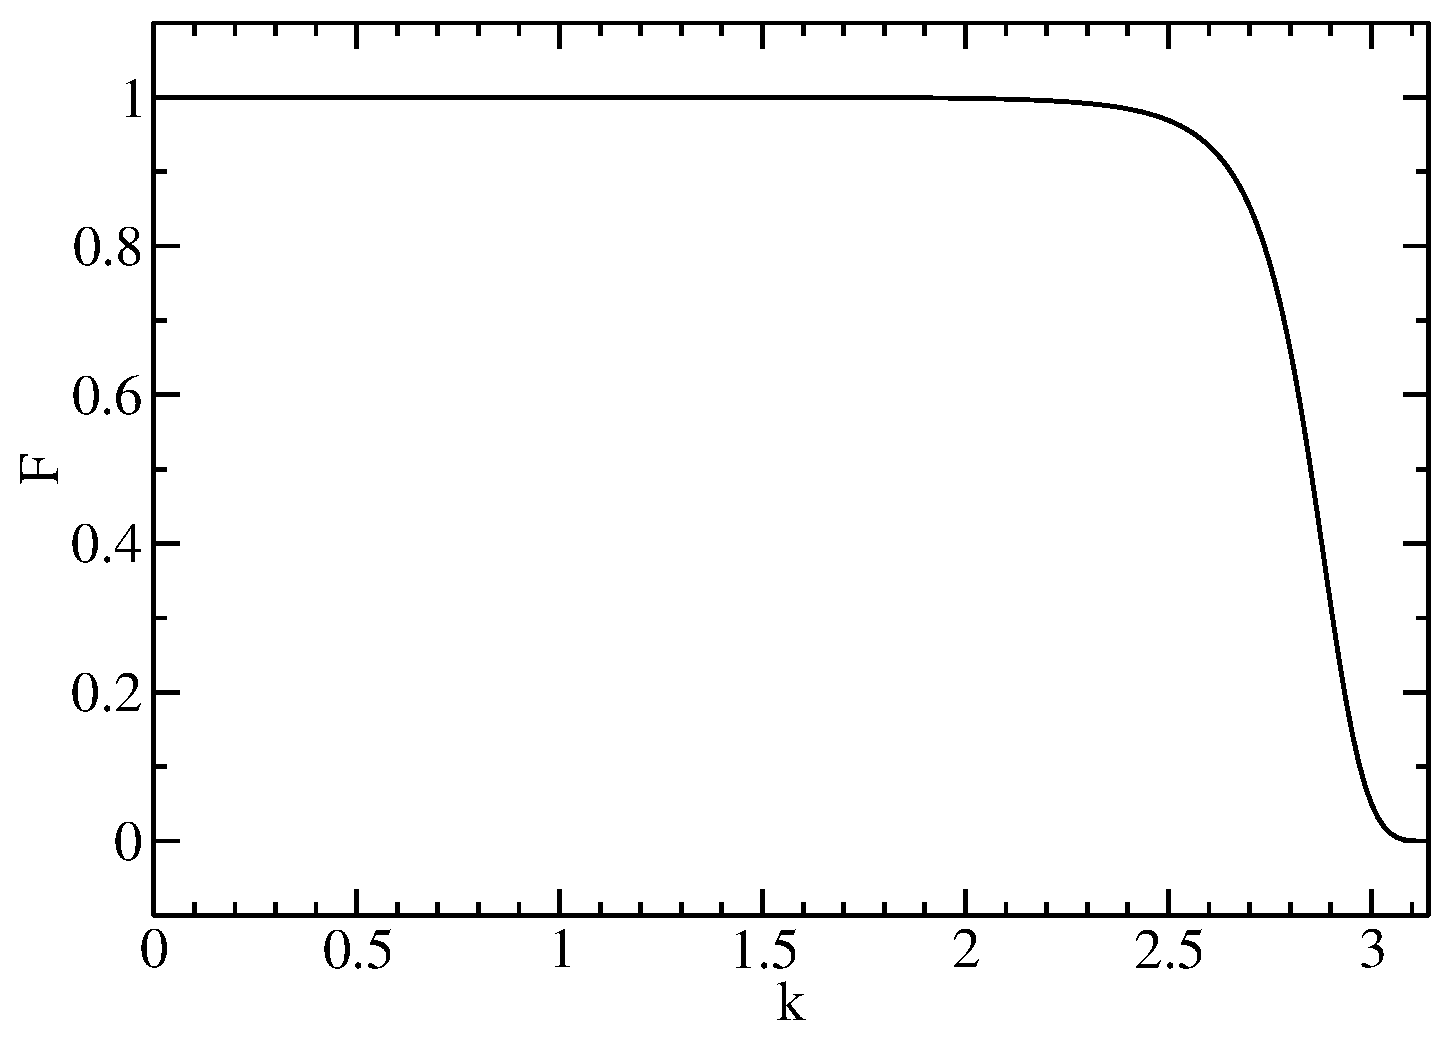
\includegraphics[width=4in]{transfer_function}
FIXME
\end{center}
 \caption{Transfer function (\ref{eq:transfer}) of the $8^{\rm th}$ order filter defined in
 (\ref{eq:filter}) and table~\ref{tab:coefficients}.}
\label{fig:transfer}
\end{figure}

There remain three details to work out: 1) the coefficients provided by
Cook \& Cabot apparently are only given to a part in $10^6$, we will
need them specified to machine precision to retain the $8^{\rm th}$
order accuracy; 2) the filter stencil is quite wide, so that for points
near the wall, the stencil will fall outside the domain; 3) the value of
$\phi$ needs to be selected. Treatment of
these issues is discussed below.

%\paragraph{Parameter Values} The filter is defined by 7 independent
Parameter Values: The filter is defined by 7 independent
parameters, which are constrained by a number of requirements:
\begin{itemize}
\item Eighth order accuracy introduced 4 linear constraints required to
      force the $0^{\rm th}$, $2^{\rm nd}$, $4^{\rm th}$ and $6^{\rm
      th}$
      order errors to zero. Odd order errors are zero by symmetry.
\item The Transfer function should be zero at $\hat k=\pi$, and ideally
      it would have a number of zero derivatives at $\pi$. The odd order
      derivatives are zero by symmetry. We can thus force the second
      derivative of the transfer function to be zero. This amounts to
      two more linear constraints
\item This leaves a 1-parameter family of transfer functions, where that
      parameter can presumably be used to adjust the location of the
      cut-off.
\end{itemize}
High precision values of the coefficients can thus be obtained by
solving the constraint equations. The order of accuracy constraints are:
\begin{eqnarray}
\sum_{i=0}^2\alpha_i&=&\sum_{i=0}^4a_i\\
\sum_{i=0}^2i^2\alpha_i&=&\sum_{i=0}^4i^2a_i\\
\sum_{i=0}^2i^4\alpha_i&=&\sum_{i=0}^4i^4a_i\\
\sum_{i=0}^2i^6\alpha_i&=&\sum_{i=0}^4i^6a_i
\end{eqnarray}
The constraints on the transfer function at $\hat k=\pi$ are:
\begin{eqnarray}
0&=&\sum_{i=0}^4a_i(-1)^i\\
0&=&\sum_{i=0}^4a_i i^2 (-1)^i
\end{eqnarray}
As it happens, all six of these equations are satisfied exactly by the
coefficients in the table. These values can thus be used, and we can defer finding other
members of the family of filters until later.

%\paragraph{Wall Treatment} There are three fairly straight-forward
Wall Treatment: There are three fairly straight-forward
approaches to filtering at the walls:
\begin{enumerate}
\item Just don't apply the filter operator for points near the
      wall. Since the filter stencil is broad, this would mean that the
      four collocation points closest to the wall would not have the
      filter applied.
\item Allow the filter kernel to spill out of the domain, with the
      external points having values obtained in some way. Victor
      suggests reflecting the solution through the wall, which ensures
      that the extended solution is continuous with continuous first
      derivatives. But the second derivatives will be discontinuous.
\item Us a one-sided high order filter at points near the wall.
\end{enumerate}
It is proposed that we start with approach (1) near the wall, and
approach (2) in the free stream. Approach (3) would need to be
formulated and will be deferred to later, in case (1) and (2)  are not
sufficient. The properties of these two approaches should be evaluated
by analyzing the eigenvalues and eigenvectors of the resulting
finite-domain $F$ operator.

%\paragraph{Selecting the value of $\phi$}
Selecting the value of $\phi$:
One wants to select $\phi$ sufficiently large so that the high
wavenumbers are effectively damped (eliminated), but not so large as to
cause significant damping for physically relevant wavenumbers. One
reasonable way to accomplish this is to note that by definition, since
this is for DNS, viscous (molecular) damping at the highest wavenumbers
is sufficient. For uniform knots and constant diffusivity, this would
suggest a value of $\phi$ of order $\pi^2\nu/\Delta y^2$, where $\nu$ is
the diffusivity (e.g. kinematic viscosity for momentum). However, this
is not the case. One possibility would thus be to make $\phi$ a function
of $y$, based on say an approximate $\nu$ representing the mean, and the
actual knot or collocation point locations. The eigen characteristics of
the resulting operator $\phi(F-I)$ in (\ref{eq:time_filter}) should also
be evaluated. Victor's experience in Comp regarding this would be useful.

\subsection{Viscous Filter}
In addition to the Cook and Cabot filter, a filter source based on the
difference between the ``real'' B-spline second derivative operator
and repeated application of the first derivative operator will be
investigated.  The primary goal of this filter choice is to avoid a
mismatch in the spectrum between the full discrete viscous operator
and the viscous contribution in the linear operator (see
\S\ref{sec:discretization} and~\S\ref{sec:implicit} for specification
of these operators).  This mismatch would make the explicit part of
the operator anti-diffusive, which can adversely effect the largest
stable time step if strong enough.  
\todo{Reference Rhys' analysis of using max vs. mean viscosity for
  reference profile in implicit operator to back this up.}

For clarity, we first describe the scheme for the following scalar
evolution equation:
%
\begin{equation*}
\pp{u}{t} = \pp{G_{visc}}{y},
\end{equation*}
% 
where $G_{visc} = \nu(u) \partial u / \partial y$.  In this case,
the ``flux-based'' B-spline collocation scheme takes the following
form
%
\begin{equation}
\label{eqn:flux_form_scalar_nofilter}
M \pp{U}{t} = D_1 M^{-1} G,
\end{equation}
% 
where $U$ is the vector of B-spline coefficients, $M$ is the mass
matrix (taking coefficients to collocation point values), $D_1$ is the
B-spline first derivative operator (taking coefficients to collocation
point derivative values).  The vector $G$ is the flux
evaluated at the collocation points, which can be written
%
\begin{equation*}
G = N D_1 U,
\end{equation*}
% 
where $N$ is the diagonal matrix containing the viscosity evaluated
at the collocation points on its diagonal.

The filter source is given by adding and subtracting different
discretizations of $\nu^* \partial^2 u / \partial y^2$
from~\eqref{eqn:flux_form_scalar_nofilter}, where $\nu^*$ is a
reference profile of the viscosity $\nu$.  Specifically,
%
\begin{equation}
\label{eqn:flux_form_scalar_wfilter}
M \pp{U}{t} = D_1 M^{-1} G + N^* (D_2 - D_1 M^{-1} D_1) U,
\end{equation}
% 
where $D_2$ is the B-spline second derivative operator and $N^*$ is
a diagonal matrix with the reference profile of $\nu$ on the diagonal.

To get the filter for the full Navier-Stokes equations, this scheme is
applied to each governing equation individually using the diagonal
linearized viscous operator derived in \S\ref{sec:implicit}.



\section{Implicit Formulation}
\input{reacting_inputs/implicit_formulation.tex}

\section{Boundary Conditions and Implementation}

\todo{Edit the following for dimensional, reacting formulation}

\subsection{Wall Conditions}
At wall boundaries, mass fractions on $N_s -1$ species, temperature,
and velocity are set.  Since the mixture density is allowed to vary,
these conditions take the following form in terms of the conserved
state used in Suzerain:
%
\begin{align*}
\rho_{\alpha} &= \rho c_{\mathrm{wall},\alpha}, \quad \mathrm{for} \,\, \alpha = 2, \ldots, N_s\\
\rho u_i &= \rho u_{\mathrm{wall},i}, \quad \mathrm{for} \,\, i = 1, 2, 3 \\
\rho E &= \rho E_{\mathrm{wall}},
\end{align*}
%
where $c_{\mathrm{wall},\alpha}$ and $u_{\mathrm{wall},i}$ are the user-supplied
mass fractions and wall velocities, respectively.  The energy at the
wall $E_{\mathrm{wall}}$ is computed from these values and a
user-specified wall temperature $T_{\mathrm{wall}}$.  Specifically,
%
\begin{equation*}
E_{\mathrm{wall}} = e_{tot}(c_{\mathrm{wall},\alpha}, T_{\mathrm{wall}}) + \frac{1}{2} u_{\mathrm{wall},i} u_{\mathrm{wall},i},
\end{equation*}
%
where the mixture internal energy is
%
\begin{equation*}
e_{tot}(c_{\mathrm{wall},\alpha}, T_{\mathrm{wall}}) = \sum_{s=1}^{N_s} c_{\mathrm{wall},s} e_{s,tot}(T_{\mathrm{wall}}),
\end{equation*}
%
and $e_{s,tot}$ is the internal energy of species $s$, which depends
only on the temperature.  


\subsection{Nonreflecting freestream boundary conditions}
\label{sec:nonreflectingbcs}

\todo{Starting with Rhys' derivation, adapting the matrices to multispecies}

When simulating problems on semi-infinite domains, such as flat plates,
Suzerain requires nonreflecting freestream boundary conditions.  Without these,
acoustic waves generated by the flow cannot be leave the domain.   The trapped
acoustics pile up causing a non-physical partition of energy and spoiling the
simulated statistics.

Following \citet{Engquist1977Absorbing},
\citet{Giles1988Nonreflecting,Giles1990Nonreflecting} developed localized,
approximate two-dimensional, unsteady nonreflecting boundary conditions for the
Euler equations.  Giles' boundary conditions are adopted over the ``locally
one-dimensional inviscid'' relations of \citet{Poinsot1992Boundary} because
other codes with similar numerics have successfully employed Giles' conditions
for our problems of interest.  While \citet{Rowley2000Discretely} present
higher order techniques expected to perform better than Giles' approach, what
they describe is considerably more complex to implement.
\citet{Saxer1993QuasiThreeDimensional} extended the technique to three
dimensions but with a presentation aimed towards transonic axial flow
turbomachinery computations.  \citet{Guarini1998} summarizes the Cartesian
extension of Giles' approach to three spatial dimensions without reproducing
the associated analysis.  \citet{Medida2007} lucidly catalogs the intermediate
results necessary in three dimensions.

We now review Giles' approach following Guarini's presentation with the goal of
setting notation suitable for presenting and manipulating Medida's results for
nonreflecting $x$ boundaries in three-dimensional, Cartesian coordinates.  For
complete details, especially motivations and proofs, the work of Giles, Medida,
and Guarini should be consulted in that respective order.

For the state vector
\begin{subequations}
\label{eq:eulerprim}
\begin{align}
  U &= \left\{ \rho_\alpha, u, v, w, p \right\}
\end{align}
the Euler equations, using the ideal gas equation of state
\begin{align}
  \rho a^2 &= \gamma p,
\end{align}
may be written as follows:
\begin{align}
    \frac{\partial}{\partial{}t}U
+ A \frac{\partial}{\partial{}x}U
+ B \frac{\partial}{\partial{}y}U
+ C \frac{\partial}{\partial{}z}U
&= 0
\end{align}
\begin{align}
 A &= \begin{bmatrix}
        u & \rho_\alpha & 0 & 0 & 0              \\
        0 & u           & 0 & 0 & \frac{1}{\rho} \\
        0 & 0           & u & 0 & 0              \\
        0 & 0           & 0 & u & 0              \\
        0 & \gamma p    & 0 & 0 & u              \\
       \end{bmatrix}
&
 B &= \begin{bmatrix}
        v & 0 & \rho_\alpha & 0 & 0              \\
        0 & v & 0           & 0 & 0              \\
        0 & 0 & v           & 0 & \frac{1}{\rho} \\
        0 & 0 & 0           & v & 0              \\
        0 & 0 & \gamma p    & 0 & v              \\
       \end{bmatrix}
&
 C &= \begin{bmatrix}
        w & 0 & 0 & \rho_\alpha & 0              \\
        0 & w & 0 & 0           & 0              \\
        0 & 0 & w & 0           & 0              \\
        0 & 0 & 0 & w           & \frac{1}{\rho} \\
        0 & 0 & 0 & \gamma p    & w              \\
       \end{bmatrix}
\end{align}
\end{subequations}
% This system of equations identically describes the behavior of an analogous
% $U^*$ whenever all of
% \begin{align}
% \label{eq:eulerprimnondim}
% U^{*} &= \left\{
%   \frac{\rho}{\rho_0},
%   \frac{u}{u_0},
%   \frac{v}{u_0},
%   \frac{w}{u_0},
%   \frac{p}{\rho_0 u_0^2}
% \right\}
% &
% t_0 &= \frac{l_0}{u_0}
% &
% a_0 &= u_0
% \end{align}
% hold.  Therefore, all dimensional results obtained for $U$ remain unchanged
% in the setting of $U^*$.

Consider perturbations
\[
\delta{}U = \left\{ \delta{}\rho_\alpha, \delta{}u,
\delta{}v, \delta{}w, \delta{}p \right\}
\]
taken about some steady,
uniform reference state $\bar{U}$ so that
\[
U = \bar{U} + \delta{}U.
\]
The short-time evolution of such perturbations is governed by the linearized
Euler equations
\begin{align}
\label{eq:dimeulerperturb}
               \frac{\partial}{\partial{}t}\delta{}U
+ \bar{A} \frac{\partial}{\partial{}x}\delta{}U
+ \bar{B} \frac{\partial}{\partial{}y}\delta{}U
+ \bar{C} \frac{\partial}{\partial{}z}\delta{}U
&= 0
\end{align}
where matrices $\bar{A}$, $\bar{B}$, and $\bar{C}$ are evaluated
at $\bar{U}$.  This linearized system satisfies the prerequisites for
Giles' analysis.  Assuming a solution of the form
\begin{align}
  \delta{}U &= e^{\ii\left(
    k_x x + k_y y + k_z z - \omega t
  \right)}
  \delta\hat{U}^R
\end{align}
and substituting into the linearized equations reduces the equations to
\begin{align}
\label{eq:dimeulerreduced}
  \ii\left( - \omega I
            + k_x \bar{A}
            + k_y \bar{B}
            + k_z \bar{C}
  \right)
  \delta\hat{U}^R &= 0
\end{align}
which has nontrivial solutions only if the so-called dispersion relation
\begin{align}
  \det \left( - \omega I
              + k_x \bar{A}
              + k_y \bar{B}
              + k_z \bar{C}
       \right) &= 0
\end{align}
holds.  Defining $\lambda_x = k_x/\omega$, $\lambda_y = k_y/\omega$, and
$\lambda_z/\omega$, the dispersion relation may be equivalently expressed as
\begin{align}
\label{eq:dimeulerdisp}
  \det \left( - I
              + \lambda_x \bar{A}
              + \lambda_y \bar{B}
              + \lambda_z \bar{C}
       \right) &= 0
  .
\end{align}
Assuming $\bar{A}$ is invertible and applying
$-\left(\ii\omega{}\bar{A}\right)^{-1}$ to
equation~\eqref{eq:dimeulerreduced}, one finds an eigenvalue problem in
$\lambda_x$
\begin{align}
  \left(   \bar{A}^{-1}
         - \lambda_x I
         - \lambda_y \bar{A}^{-1} \bar{B}
         - \lambda_z \bar{A}^{-1} \bar{C}
  \right) \delta\hat{U}^R = 0
\end{align}
where $\delta\hat{U}^R$ is the eigenvector and a solution to the right null
space problem.  The signs of the associated eigenvalues, determined using the
magnitude of $\bar{u}$ relative to $\bar{a}$, are required to determine how
many characteristics are entering or exiting through the boundary.  The left
null space problem
\begin{align}
\label{eq:dimeulereigenprob}
  V^{L}
  \left(   \bar{A}^{-1}
         - \lambda_x I
         - \lambda_y \bar{A}^{-1} \bar{B}
         - \lambda_z \bar{A}^{-1} \bar{C}
  \right) &= 0
\end{align}
naturally gives rise to the associated left null vector $V^L$.  Giles,
following Engquist and Majda, used several orthogonality properties to build
the exact, nonreflecting boundary conditions
\begin{align}
\label{eq:dimeulerexact}
  V_n^L \delta{}U &= 0
\end{align}
for each $V_n^L = V^L\!\left(k_{x_n}\right)$ corresponding to \textit{either
incoming or outgoing waves}.  This exact condition is approximated using a
Taylor series in $\lambda_y$ and $\lambda_z$ for reasons of computational
tractability.  Truncating the series is equivalent to assuming waves have a
small angle of incidence to the boundary.  To first order,
\begin{align}
  \left.V_n^L\right|_{\lambda_y,\lambda_z=0}
  \delta{}U
  +
  \lambda_y
  \left.\frac{dV_n^L}{d\lambda_y}\right|_{\lambda_y,\lambda_z=0}
  \delta{}U
  +
  \lambda_z
  \left.\frac{dV_n^L}{d\lambda_z}\right|_{\lambda_y,\lambda_z=0}
  \delta{}U
  &\approx 0
  .
\end{align}
As noted by \citet{Engquist1977Absorbing} and later expounded upon by
\citet{Trefethen1986Wellposedness}, only particular higher-order series
truncations of this form lead to well-posedness.  Moreover, the straightforward
application of even this first order approximation requires either
ad~hoc~\citep{Giles1988Nonreflecting,Medida2007} or
systematic~\citep{Rowley2000Discretely} modification to produce well-behaved
inflow constraints.  Multiplying through by $-\ii\omega$, Fourier transforming
in both time and space, and using that $\bar{U}$ and therefore $V_n^L$ are both
steady and uniform yields
\begin{align}
\label{eq:dimeulerapprox}
  \frac{\partial}{\partial{}t}
  V^L
  \delta{}U
  &\approx
  \frac{dV^L}{d\lambda_y}
  \frac{\partial}{\partial{}y}\delta{}U
  +
  \frac{dV^L}{d\lambda_z}
  \frac{\partial}{\partial{}z}\delta{}U
\end{align}
where the cumbersome $\lambda_y,\lambda_z=0$ and subscript $n$ are herein
and henceforth suppressed.  Inserting ${V^L}^{-1} V^L$,
\begin{align}
  \frac{\partial}{\partial{}t}
  V^L
  \delta{}U
  &\approx
  \frac{dV^L}{d\lambda_y}
  {V^L}^{-1}
  \frac{\partial}{\partial{}y}
  V^L
  \delta{}U
  +
  \frac{dV^L}{d\lambda_z}
  {V^L}^{-1}
  \frac{\partial}{\partial{}z}
  V^L
  \delta{}U
.
\end{align}
Defining characteristic variables using the action of $V^L$, \textit{viz.}
\begin{align}
  \delta{}C &= V^L \delta{}U
  ,
\end{align}
allows writing a more compact form
\begin{align}
\label{eq:dimeulerapproxchar}
  \frac{\partial}{\partial{}t}
  \delta{}C
  &\approx
  B^G
  \frac{\partial}{\partial{}y}
  \delta{}C
  +
  C^G
  \frac{\partial}{\partial{}z}
  \delta{}C
\end{align}
employing the notation
\begin{align}
\label{eq:dimeulerapproxBG}
  B^G
&=
  \frac{dV^L}{d\lambda_y}
  {V^L}^{-1}
&
  C^G
&=
  \frac{dV^L}{d\lambda_z}
  {V^L}^{-1}
\end{align}
where the superscript $G$ is meant to suggest ``Giles''.  This last statement
intermixes the constraints for inflow and outflow conditions.  While the
submatrices vary depending on the choices made to express $V^L$ and the
magnitude of $\bar{u}$ relative to $\bar{a}$, in complete generality the matrix
equation~\eqref{eq:dimeulerapproxchar} may be partitioned as
\begin{align}
\label{eq:dimeulerapproxcharpart}
\renewcommand*{\arraystretch}{1.2}
  \frac{\partial}{\partial{}t}
  \left[\begin{array}{c}\delta{}C_{I}\\\hline\delta{}C_{O}\end{array}\right]
  &\approx
\renewcommand*{\arraystretch}{1.2}
  \left[\begin{array}{c} B^G_{I} \\ \hline B^G_{O} \end{array}\right]
  \frac{\partial}{\partial{}y}
  \delta{}C
  +
  \left[\begin{array}{c} C^G_{I} \\ \hline C^G_{O} \end{array}\right]
  \frac{\partial}{\partial{}z}
  \delta{}C
\end{align}
where subscripts $I$ and $O$ denote inflow or outflow condition submatrices,
respectively.  Only the conditions arising from one set of submatrices are to
be applied at any location.  The ``other'' submatrices are defined to be zero
depending on the use case at hand:
\begin{align}
  B^G &=
\renewcommand*{\arraystretch}{1.2}
  \left[\begin{array}{c} B^G_{I} \\ \hline 0       \end{array}\right]
  &
  C^G &=
\renewcommand*{\arraystretch}{1.2}
  \left[\begin{array}{c} C^G_{I} \\ \hline 0       \end{array}\right]
  &
  &\left(\text{inflow boundary}\right)
\\
  B^G &=
\renewcommand*{\arraystretch}{1.2}
  \left[\begin{array}{c} 0       \\ \hline B^G_{O} \end{array}\right]
  &
  C^G &=
\renewcommand*{\arraystretch}{1.2}
  \left[\begin{array}{c} 0       \\ \hline C^G_{O} \end{array}\right]
  &
  &\left(\text{outflow boundary}\right)
\end{align}
Notationally, it will later be convenient to have a projection
\begin{align}
\label{eq:PG}
\renewcommand*{\arraystretch}{1.2}
  P^G
  &=
  \left[\begin{array}{c} P^G_{I} \\ \hline P^G_{O} \end{array}\right]
\end{align}
defined to preserve only the characteristic(s) constrained by a boundary
condition with the ``other'' submatrix again being zero.  This definition
implies
\begin{align}
\label{eq:PGidempotence}
  P^G B^G &= B^G
  &
  P^G C^G &= C^G
.
\end{align}
Notice $I - P^G$ recovers the characteristics \emph{not} constrained by the
boundary condition For some $\bar{U}$ possessing an agreed upon relationship
between $\bar{u}$ and $\bar{a}$, specifying $V^L$ and these partitioned
submatrices concretely states a Giles-like nonreflecting $x$ boundary condition
for the Euler equations.

In section 5.8 of his thesis, Medida presents two such concrete nonreflecting
boundary condition specifications for subsonic inflows and outflows where $0 <
\bar{u} < \bar{a}$.  Medida's equations~(5.78) and~(5.79) specify the
transformations to and from characteristic variables:
\begin{align}
\label{eq:dimeulerapproxmedidaproj}
  V^L &= \left[\begin{array}{ccccc}
    -\bar{a}^2 & 0                   & 0                  & 0                  & c_\alpha \\ \noalign{\smallskip}
    0          & 0                   & \bar{\rho} \bar{a} & 0                  & 0 \\ \noalign{\smallskip}
    0          & 0                   & 0                  & \bar{\rho} \bar{a} & 0 \\ \noalign{\smallskip}
    0          & \bar{\rho} \bar{a}  & 0                  & 0                  & 1 \\ \noalign{\smallskip}
    0          & -\bar{\rho} \bar{a} & 0                  & 0                  & 1 \\ \noalign{\smallskip}
  \end{array}\right]
&  % COMPUTE THIS (Seguir aca...)
  {V^L}^{-1} &= \left[\begin{array}{ccccc}
    -\frac{c_\alpha}{\bar{a}^2} & 0                            & 0                            & \frac{c_\alpha}{2\bar{a}^2}   & \frac{c_\alpha}{2\bar{a}^2}     \\ \noalign{\smallskip}
    0                           & 0                            & 0                            & \frac{1}{2\bar{\rho} \bar{a}} & - \frac{1}{2\bar{\rho} \bar{a}} \\ \noalign{\smallskip}
    0                           & \frac{1}{\bar{\rho} \bar{a}} & 0                            & 0                             & 0                               \\ \noalign{\smallskip}
    0                           & 0                            & \frac{1}{\bar{\rho} \bar{a}} & 0                             & 0                               \\ \noalign{\smallskip}
    0                           & 0                            & 0                            & \frac{1}{2}                   & \frac{1}{2}                     \\ \noalign{\smallskip}
  \end{array}\right]
\end{align}
For the single species case ($c_\alpha$=1), direct computation shows
\[
  \det V^L = -2\bar{\rho}^3\bar{a}^5
\]
and so $V^L$ is always nonsingular for a realizable reference state.  Medida's
equations~(5.82) and~(5.83) provide one pair of inflow and outflow conditions
for which reflection coefficients were not reported:
\todo{Extend expression of $B^G$ and $C^G$ for multispecies flow}
%
\begin{align} \label{eq:dimeulerapproxmedidaopt1} B^G_1 &=
\left[\begin{array}{ccccc} 0 & 0                         & 0       & 0
& 0                         \\ \noalign{\smallskip} 0 & \bar{v}
& 0       & \frac{\bar{a} + \bar{u}}{2} & \frac{\bar{a}-\bar{u}}{2} \\
\noalign{\smallskip} 0 & 0                         & \bar{v} & 0
& 0                         \\ \noalign{\smallskip} 0 &
\frac{\bar{a}-\bar{u}}{2} & 0       & \bar{v}                     & 0
\\ \noalign{\smallskip} \hline 0 & \bar{u}                   & 0       & 0
& \bar{v}                   \\ \noalign{\smallskip} \end{array}\right] & C^G_1
&= \left[\begin{array}{ccccc} 0 & 0       & 0                         & 0
& 0                         \\ \noalign{\smallskip} 0 & \bar{w} & 0
& 0                         & 0                         \\
\noalign{\smallskip} 0 & 0       & \bar{w}                   &
\frac{\bar{a}+\bar{u}}{2} & \frac{\bar{a}-\bar{u}}{2} \\ \noalign{\smallskip}
0 & 0       & \frac{\bar{a}-\bar{u}}{2} & \bar{w}                   & 0
\\ \noalign{\smallskip} \hline 0 & 0       & \bar{u}                   & 0
& \bar{w}                   \\ \noalign{\smallskip} \end{array}\right]
\end{align}
%
where partitioning has been used to delineate inflow versus outflow submatrices
within $B^G$ and $C^G$.  
The characteristic-preserving projection operator is
%
\begin{align}
\label{eq:PGmedida}
  P^G
  &= \left[\begin{array}{ccccc}
    1 & 0 & 0 & 0 & 0 \\
    0 & 1 & 0 & 0 & 0 \\
    0 & 0 & 1 & 0 & 0 \\
    0 & 0 & 0 & 1 & 0 \\ \hline
    0 & 0 & 0 & 0 & 1 \\
  \end{array}\right]
.
\end{align}
%
We assume, but have not verified, analysis like that presented in
\citet[\textsection{}3.7.4]{Giles1988Nonreflecting} extends to Medida's
analogous results.  At the inflow, the outgoing pressure wave produces no
reflected entropy or vorticity waves and generates a fourth-order pressure
reflection.  At the outflow, the outgoing entropy and vorticity waves produce
no reflections while the outgoing pressure wave produces a second order
reflection.  In contrast, Medida's equation~(5.84), which arises from modifying
the already-well-posed outflow condition to match the well-posed inflow
condition, provides different outflow submatrices:
\todo{Extend expression of $B^G_2$ and $C^G_2$ for multispecies flow}
\begin{align}
\label{eq:dimeulerapproxmedidaopt2}
  B^G_2 &= \left[\begin{array}{ccccc}
    0 & 0                         & 0       & 0                           & 0                         \\ \noalign{\smallskip}
    0 & \bar{v}                   & 0       & \frac{\bar{a} + \bar{u}}{2} & \frac{\bar{a}-\bar{u}}{2} \\ \noalign{\smallskip}
    0 & 0                         & \bar{v} & 0                           & 0                         \\ \noalign{\smallskip}
    0 & \frac{\bar{a}-\bar{u}}{2} & 0       & \bar{v}                     & 0                         \\ \noalign{\smallskip} \hline \noalign{\smallskip}
    0 & \frac{\bar{a}+\bar{u}}{2} & 0       & 0                           & \bar{v}                   \\ \noalign{\smallskip}
  \end{array}\right]
&
  C^G_2 &= \left[\begin{array}{ccccc}
    0 & 0       & 0                         & 0                         & 0                         \\ \noalign{\smallskip}
    0 & \bar{w} & 0                         & 0                         & 0                         \\ \noalign{\smallskip}
    0 & 0       & \bar{w}                   & \frac{\bar{a}+\bar{u}}{2} & \frac{\bar{a}-\bar{u}}{2} \\ \noalign{\smallskip}
    0 & 0       & \frac{\bar{a}-\bar{u}}{2} & \bar{w}                   & 0                         \\ \noalign{\smallskip} \hline \noalign{\smallskip}
    0 & 0       & \frac{\bar{a}+\bar{u}}{2} & 0                         & \bar{w}                   \\ \noalign{\smallskip}
  \end{array}\right]
\end{align}
At the outflow, these matrices cause outgoing pressure waves to produce fourth
and first order reflections, respectively.  As Giles
notes~\citep{Giles1990Nonreflecting}, this second outflow condition is
preferable only when one knows there will be no outgoing vorticity wave.  This
should be the case for some of our problems of interest.

In section~4.3 of his thesis, \citet{Guarini1998} proved the linear
structure of the Euler equations admits a straightforward translation of Giles'
boundary conditions to another set of state variables $V$ with steady, uniform
reference state $\bar{V}$ and therefore perturbations
\[
  \delta{}V = V - \bar{V}.
\]
The corresponding coordinate transformation Jacobian matrix is
\[
   S = \frac{\partial{}U}{\partial{}V}
   .
\]
In this new setting, Guarini rewrote the exact nonreflecting
conditions~\eqref{eq:dimeulerexact} as
\begin{align}
  \left(V^L S\right) \delta{}V &= 0
\end{align}
which causes the approximate condition~\eqref{eq:dimeulerapprox} to become
\begin{align}
\label{eq:dimeulertransform}
  V^L
  S
  \frac{\partial}{\partial{}t}
  \delta{}V
  &\approx
  \frac{dV^L}{d\lambda_y}
  S
  \frac{\partial}{\partial{}y}
  \delta{}V
  +
  \frac{dV^L}{d\lambda_z}
  S
  \frac{\partial}{\partial{}z}
  \delta{}V
  .
\end{align}
Using notation from the compact representation~\eqref{eq:dimeulerapproxBG},
\begin{align}
\label{eq:dimeulertransformcharnot}
  V^L S
  \frac{\partial}{\partial{}t}
  \delta{}V
  &\approx
  B^G V^L S
  \frac{\partial}{\partial{}y}
  \delta{}V
  +
  C^G V^L S
  \frac{\partial}{\partial{}z}
  \delta{}V
\end{align}
is the simplest form for applying Medida's $x$ boundary condition matrices to
alternative state variables.

The particular coordinate transformation Suzerain requires maps the dimensional
primitive state $U$ satisfying requirements~\eqref{eq:eulerprimnondim} to the
conserved state $V$ (dimensional) and~\ref{nondim_equations}:
%
\begin{align}
\label{eq:multieulerconsdim}
V
= \left\{
    \rho_\alpha,
    \rho,
  \,\rho u,
  \,\rho v,
  \,\rho w,
  \,\rho E
\right\}
\end{align}
%
where in this case $\alpha$ spans from 1 to $N_s$-1.
The relationships between $U$ and $V$ allows computing the Jacobian matrix
evaluated at some $\bar{V}$.  For total energy, a simplified expression that
resembles the single species case can be obtained if we consider a linearized
expression for internal energy. In general the total energy is given by
%
\begin{equation}
\rho E = \rho e_{tot}(c_\alpha, T) + \frac{1}{2} \rho \left( u^2 + v^2+ w^2 \right)
\end{equation}
%
with 
%
\begin{equation}
\begin{split}
e_{tot}(c_s, T) 
&= \sum_{s=1}^{N_s} c_s e_{s,tot}(T)  \\
&= \sum_{s=1}^{N_s} c_s e_{s,int}(T) + \sum_{s=1}^{N_s} c_s h^0_s 
\end{split}
\end{equation}
%

Expanding in a Taylor series to first order about $(c_{s,0},T_0)$ we get
%
\begin{equation}
\begin{split}
e_{tot}(c_s, T) 
&\approx e_{tot}(c_{s,0}, T_0) 
 + \pp{e_{tot}}{T} (T-T_0) + \sum_{s=1}^{N_s} \pp{e_{tot}}{c_s} (c_s-c_{s,0})\\
&= e_{tot,0}
 + C_{v,\text{mix},0} (T-T_0) + \sum_{s=1}^{N_s} c_s e_{s,tot,0} - \sum_{s=1}^{N_s}  c_{s,0} e_{s,tot,0} \\
&= C_{v,\text{mix},0}  T      + \sum_{s=1}^{N_s} c_s e_{s,tot,0} - C_{v,\text{mix},0} T_0  \\
\end{split}
\end{equation}
%
where it is implied that all the derivatives are specialized at the reference state.
Therefore, an approximate expression for total energy is obtained as
\begin{equation}
\begin{split}
\rho E 
&\approx \rho C_{v,\text{mix},0} T 
   + \rho \sum_{s=1}^{N_s} c_s e_{s,tot,0} 
   - \rho C_{v,\text{mix},0} T_0 
   + \frac{1}{2} \rho \left( u^2 + v^2+ w^2 \right) \\
&= \frac{P}{\gamma_{\text{mix},0}-1}
   + \sum_{s=1}^{N_s} \rho_s e_{s,tot,0} 
   - \frac{P_0}{\gamma_{\text{mix},0}-1}
   + \frac{1}{2} \sum_{s=1}^{N_s} \rho_s \left( u^2 + v^2+ w^2 \right)
\end{split}
\end{equation}

The Jacobian is then
\todo{Make size of matrices consistent through the derivation}
\begin{align}
S &= 
\left[\begin{array}{cccccc}
    1      % 11
  & 0      % 12
  & 0      % 13
  & 0      % 14
  & 0      % 15
  & 0      % 16
  \\ \noalign{\medskip}
   -1      % 21
  & 1      % 22
  & 0      % 23
  & 0      % 24
  & 0      % 25
  & 0      % 26
  \\ \noalign{\medskip}
    0                                % 31
  & - \frac{\bar{u}}{\bar{\rho}}     % 32
  & \frac{1}{\bar{\rho}}             % 33
  & 0                                % 34
  & 0                                % 35
  & 0                                % 36
  \\ \noalign{\medskip}
    0                                % 41
  & - \frac{\bar{v}}{\bar{\rho}}     % 42
  & 0                                % 43
  & \frac{1}{\bar{\rho}}             % 44
  & 0                                % 45
  & 0                                % 46
  \\ \noalign{\medskip}
    0                                % 51
  & - \frac{\bar{w}}{\bar{\rho}}     % 52
  & 0                                % 53
  & 0                                % 54
  & \frac{1}{\bar{\rho}}             % 55
  & 0                                % 56
  \\ \noalign{\medskip}
    \left(\bar{\gamma} - 1\right) \left(-\bar{e}_{1,tot}+\bar{e}_{d,tot}\right) % 61
  & \left(\bar{\gamma} - 1\right) 
    \left(-\bar{e}_{d,tot} + 
    0.5 \left(\bar{u}^2 + \bar{v}^2 + \bar{w}^2\right)
    \right) % 62
  & \left(1 - \bar{\gamma}\right) \bar{u}       % 63
  & \left(1 - \bar{\gamma}\right) \bar{v}       % 64
  & \left(1 - \bar{\gamma}\right) \bar{w}       % 65
  & \bar{\gamma}-1                              % 66
  \\ \noalign{\medskip}
\end{array}\right]
,
\end{align}
%
where $\bar{e}_{d,tot}$ is the total specific energy of the diluter species.
The inverse is
\begin{align}
S^{-1} &= \left[\begin{array}{cccccc}
  1         & 0         & 0          & 0            & 0            & 0 \\
  1         & 1         & 0          & 0            & 0            & 0 \\
  \bar{u}   & \bar{u}   & \bar{\rho} & 0            & 0            & 0 \\
  \bar{v}   & \bar{v}   & 0          & \bar{\rho}   & 0            & 0 \\
  \bar{w}   & \bar{w}   & 0          & 0            & \bar{\rho}   & 0 \\
  \bar{e}_{1,tot} + 0.5 \left( \bar{u}^2 + \bar{v}^2 + \bar{w}^2\right)
& \bar{e}_{2,tot} + 0.5 \left( \bar{u}^2 + \bar{v}^2 + \bar{w}^2\right)
& \bar{\rho} \bar{u} 
& \bar{\rho} \bar{v} 
& \bar{\rho} \bar{w} 
& \frac{1}{\bar{\gamma}-1}
\end{array}\right]
.
\end{align}
% Medida's matrices $V^L$, $B^G$, and $C^G$ derived for $U$ remain valid for
% nondimensional $U^*$ possessing sound speed $a/u_0$.  When reusing these
% matrices for $V^*$ every sound speed must be scaled by $1/\Mach$ because
% \[
%   \frac{\bar{a}}{u_0} = \frac{a_0 \bar{a}^*}{u_0} = \frac{\bar{a}^*}{\Mach}.
% \]

Thus far nonreflecting $x$ boundary conditions in physical space have been
presented.  Suzerain requires rotating these results to handle nonreflecting
$y$ boundaries followed by transforming the constraints into coefficient space.
Defining
\begin{align}
  x' &= z &
  y' &= x &
  z' &= y
\intertext{
induces the following relationships:
}
  u &= v' &
  v &= w' &
  w &= u'
\\
  \frac{\partial}{\partial{}x} &= \frac{\partial}{\partial{}y'} &
  \frac{\partial}{\partial{}y} &= \frac{\partial}{\partial{}z'} &
  \frac{\partial}{\partial{}z} &= \frac{\partial}{\partial{}x'}
\end{align}
The perturbed state vector entries may be reordered more conventionally by
defining $R^Y$ and $\delta{}V'$ per
\begin{align}
  \delta{}V
  &= \begin{bmatrix}
       \delta\rho     \\
       \delta\rho{}v' \\
       \delta\rho{}w' \\
       \delta\rho{}u' \\
       \delta\rho{}E  \\
     \end{bmatrix}
  = R^Y \delta{}V'
  = \begin{bmatrix}
      1 & 0 & 0 & 0 & 0 \\
      0 & 0 & 1 & 0 & 0 \\
      0 & 0 & 0 & 1 & 0 \\
      0 & 1 & 0 & 0 & 0 \\
      0 & 0 & 0 & 0 & 1 \\
    \end{bmatrix}
    \begin{bmatrix}
      \delta\rho     \\
      \delta\rho{}u' \\
      \delta\rho{}v' \\
      \delta\rho{}w' \\
      \delta\rho{}E  \\
    \end{bmatrix}
  .
\end{align}
Substituting these details into equation~\eqref{eq:dimeulertransformcharnot}
produces the desired nonreflecting $y$ boundary condition,
\[
\label{eq:dimeulertransformcharnotYwieldy}
\left.\left[
  V^L S
\right]\right|_{\bar{u}=\bar{v}', \bar{v}=\bar{w}', \bar{w}=\bar{u}'}
  R^Y
  \frac{\partial}{\partial{}t}
  \delta{}V'
\approx
\left.\left[
  C^G V^L S
\right]\right|_{\bar{u}=\bar{v}', \bar{v}=\bar{w}', \bar{w}=\bar{u}'}
  R^Y
  \frac{\partial}{\partial{}x'}
  \delta{}V'
  +
\left.\left[
  B^G V^L S
\right]\right|_{\bar{u}=\bar{v}', \bar{v}=\bar{w}', \bar{w}=\bar{u}'}
  R^Y
  \frac{\partial}{\partial{}z'}
  \delta{}V'
.
\]
Suppressing the primes and matrix evaluation details makes the above result
much more wieldy,
\[
\label{eq:dimeulertransformcharnotYphys}
  \left[V^L S\right]
  R^Y
  \frac{\partial}{\partial{}t}
  \delta{}V
\approx
  \left[C^G V^L S\right]
  R^Y
  \frac{\partial}{\partial{}x}
  \delta{}V
  +
  \left[B^G V^L S\right]
  R^Y
  \frac{\partial}{\partial{}z}
  \delta{}V
.
\]
Transforming to Fourier space gives a linear condition almost suitable for
implicit advance per section~\ref{sec:timediscretization},
\begin{align}
\label{eq:dimeulertransformcharnotYwave}
  \left[V^L S\right]
  R^Y
  \frac{\partial}{\partial{}t}
  \hat{V}
&\approx
  \ii k_x
  \left[C^G V^L S\right]
  R^Y
  \hat{V}
  +
  \ii k_z
  \left[B^G V^L S\right]
  R^Y
  \hat{V}
.
\end{align}
This last result holds identically for boundary collocation points and boundary
coefficients because the boundary value for a B-spline basis expansion is
nothing but the boundary coefficient.  Notice that when $k_x=k_z=0$ the
relevant characteristics within the mean state are held constant in time.

While constraint~\eqref{eq:dimeulertransformcharnotYwave} fixes the
characteristics arriving from beyond the boundary, it does not evolve the
remaining ones determined by the simulation domain.  Returning to the time
discretization of section~\ref{sec:timediscretization},
equation~\eqref{eq:timediscretization} evolves coefficients more or less like
\begin{align}
\label{eq:coeffspaceevolve}
  \frac{\partial}{\partial{}t} \hat{V} &= L \hat{V} + N(\hat{V})
  .
\end{align}
At the nonreflecting $y$ boundary, projecting the evolution into characteristic
space yields
\begin{align}
  \left[V^L S\right] R^Y
  \frac{\partial}{\partial{}t} \hat{V} &=
  \left[V^L S\right] R^Y
  \left(
    L \hat{V}
    +
    N(\hat{V})
  \right)
  .
\end{align}
Updating only the unconstrained characteristics using $P^G$ as defined
\vpageref{eq:PG},
\begin{align}
  \left(I - P^G\right)
  \left[V^L S\right] R^Y
  \frac{\partial}{\partial{}t} \hat{V}
&=
  \left(I - P^G\right)
  \left[V^L S\right] R^Y
  \left(
    L \hat{V}
    +
    N(\hat{V})
  \right)
  .
\end{align}
Applying $P^G$ to both sides of
equation~\eqref{eq:dimeulertransformcharnotYwave}, simplifying
using~\eqref{eq:PGidempotence}, and adding that to the above equality,
\begin{align}
  \left[V^L S\right]
  R^Y
  \frac{\partial}{\partial{}t}
  \hat{V}
&\approx
  \ii k_x
  \left[C^G V^L S\right]
  R^Y
  \hat{V}
  +
  \ii k_z
  \left[B^G V^L S\right]
  R^Y
  \hat{V}
\\
&{}+
  \left(I - P^G\right)
  \left[V^L S\right] R^Y
  \left(
    L \hat{V}
    +
    N(\hat{V})
  \right)
.
\end{align}
Moving the nonsingular characteristic projection to the right hand side and
collecting linear terms,
\begin{align}
\label{eq:dimeulertransformevolve}
  \frac{\partial}{\partial{}t}
  \hat{V}
&\approx
\overbrace{
  {R^Y}^{-1}
  \left[V^L S\right]^{-1}
  \left(
    \left( \ii k_x \left[C^G\right] + \ii k_z \left[B^G\right] \right)
    \left[V^L S\right] R^Y
    +
    \left(I-P^G\right)
    \left[V^L S\right] R^Y
    L
  \right)
}^{L^G}
  \hat{V}
\\
&{}+
\underbrace{
  {R^Y}^{-1}
  \left[V^L S\right]^{-1}
  \left(I - P^G\right)
  \left[V^L S\right] R^Y
  N(\hat{V})
}_{N^G\left(\hat{V}\right)}
,
\end{align}
a boundary evolution equation matching the form~\eqref{eq:coeffspaceevolve} is
recovered.  Further auxiliary definitions could improve the previous equation's
brevity but they would obfuscate the derivation and the physics.

While the derivation of this section's results has assumed a steady $\bar{V}$,
in practice $\bar{V}$ is not constant.  For example, the spatially-averaged,
instantaneous wall-normal outflow velocity generated by a homogenized boundary
layer problem may be unknown and will vary in time.  The mean state at the
beginning of the first Runge--Kutta substep should be taken as the ``steady''
$\bar{V}$ for the direction of the time step.  The mean state should be evolved
according to equation~\eqref{eq:dimeulertransformevolve} modified to account
for any auxiliary constraints (e.g. holding freestream streamwise momentum
constant at each substep).

Evidently, Giles' conditions can be shoehorned into
section~\ref{sec:imextreatment}'s IMEX Runge--Kutta framework by modifying the
action of any existing global operators $L$ and $N$ to obtain the
boundary-specific $L^G$ and $N^G$ behavior specified by
equation~\eqref{eq:dimeulertransformevolve}.  Implementing
$\left(M+\varphi{}L^G\right)\hat{V}$ in an $L$-agnostic way atop an existing
routine accumulating $\left(M+\varphi{}L\right)\hat{V}$ out-of-place is best
done by having the latter routine return $\varphi{}L\hat{V}$ so that the
incremental action of $L^G$ relative to $L$ can be further accumulated:
\begin{alignat}{10}
% Makes no sense to me that I needed to use phantom below...
% ...instead of being able to just use alignat directly.
\left(M+\varphi{}L^G\right)\hat{V} - \left(M+\varphi{}L\right)\hat{V}
  &={}   &&\ii \varphi{} k_x \, &&{R^Y}^{-1} \left[V^L S\right]^{-1} &&\left[C^G\right]                    &&\left[V^L S\right] {R^Y} &&\,\,\hat{V} \\
  &{}+{} &&\ii \varphi{} k_z    &&{R^Y}^{-1} \left[V^L S\right]^{-1} &&\left[B^G\right]                    &&\left[V^L S\right] {R^Y} &&\,\,\hat{V} \\
  &{}-{} &&                     &&{R^Y}^{-1} \left[V^L S\right]^{-1} &&\phantom{\Bigl[}P^G\phantom{\Bigr]} &&\left[V^L S\right] {R^Y} &&\left(\varphi{}L\hat{V}\right)
\end{alignat}
The auxiliary work and storage required is small and scales like two times the
number of equations as $\varphi{}L\hat{V}$ need only be returned for at most
the two boundaries of $\hat{V}$.  No special handling is required for in-place
application as it is currently implemented by incrementally applying
out-of-place routines using auxiliary buffers.  Implementing
$\left(M+\varphi{}L^G\right)^{-1}$ atop $\left(M+\varphi{}L\right)^{-1}$ is
best done by modifying the boundary equations after $M+\varphi{}L$ is formed
but before the matrix is factorized.  Doing so requires using that, for a
B-spline basis, $M$ contains only a single one in the boundary equations with
all other entries being zero.  Happily, $N^G(\hat{V})$ can be found by a
straightforward linear transformation of $N(\hat{V})$ after the latter has been
computed.  The required $C^G$-, $B^G$-, and $P^G$-related matrices may be
computed only once per nonreflecting boundary per Runge--Kutta time step from
$\bar{V}$ and then cached for repeated use.

Finally, \citet{Guarini1998} mentions that \citet{Poinsot1992Boundary}
suggest two additional viscous conditions be supplied when conditions like
these are applied to the Navier--Stokes equations.  These are currently omitted
but that choice may need to be revisited.  Guarini also rotated the
nonreflecting boundary to match the nonorthogonal coordinate system used for
his spatially-homogenized boundary layer.  Personal communications with Victor
Topalian regarding his temporally-homogenized work suggests reorienting the
nonreflecting coordinate system is unnecessary.  However, modest grid
stretching near the freestream and other ``solution conditioning'' tools like
low pass filtering have been employed in his work.  This choice, too, might
need to be reviewed.



\subsection{Characteristics from quasi-linear equations for free-stream boundary}
\todo{For reference in case the NSCBC condition are implemented}
\subsubsection{Development}
We express the system of equation in terms of primitive variables, 
$V=(u_n, u_{t_1}, u_{t_2}, P, \rho_1, \ldots, \rho_N)$, where $u$ is velocity,
$P$ is pressure, $\rho_k$ are species densities, the subindex $n$ represents the
direction normal to the boundary, and the subindices $t_1, t_2$ represent 
tangential directions to the boundary, orthogonal to each other.

Following~\citet{Moureau2005Numerical}, the system of equations can be written
as
%
\begin{align}
  \pp{}{t}V
  + E_n \pp{}{n}V
  &= T, \\
  \pp{}{t}V
  + d
  &= T,
\end{align}
%
where $d$ represents the terms with first derivative in the normal direction, 
and T represent all the other terms. $E_n$ is given by
\begin{equation}
E_n =
\left(
\begin{array}{ccccccc}
 u_n & 0 & 0 & \frac{1}{\rho} & 0 & \ldots & 0 \\
 0 & u_n & 0 & 0 & 0 & \ldots & 0 \\
 0 & 0 & u_n & 0 & 0 & \ldots & 0 \\
 \rho c^2 & 0 & 0 & u_n & 0 & \ldots & 0 \\
 \rho_1 & 0 & 0 & 0 & u_n & \ldots & 0 \\
 \vdots & \vdots & \vdots & \vdots & \vdots & \ddots & \vdots \\
 \rho_N & 0 & 0 & 0 & 0 & \ldots & u_n
\end{array}
\right)
\end{equation}

We consider now the eigendecomposition of $E_n$,
\begin{equation}
E_n = S \Lambda S^{-1},
\end{equation}
where $S$ is a square matrix, such that the $j$th column of $S$ corresponds to
the $r_j$ right eigenvector, and $\Lambda$ is a diagonal matrix where the
$j$th diagonal element is equal to the eigenvalue $\lambda_j$. This is
$\Lambda_{ij}=\delta_{ij} \lambda_j$. Therefore, we can write 
%
\begin{align}
  S^{-1} \pp{}{t}V
  +  \Lambda S^{-1} \pp{}{n}V
  &= S^{-1} T, \\
  \pp{}{t}A
  + \Lambda \pp{}{n}A
  &= T_A,
\end{align}
%
or, since $\Lambda$ is diagonal,
%
\begin{align}
  \pp{}{t}A_j
  + \lambda_j \pp{}{n}A_{\underline{j}}
  &= \left(T_A\right)_j.
\end{align}
%
The variables $A_j$ can be interptered as characteristic wave amplitudes, and
the eigenvalues $\lambda_j$ their corresponding characteristic speed.
Expanding the second term of the lhs we get
%
% \begin{equation}
% \left(
% \begin{array}{c}
% \mathcal{L}_+   \\
% \mathcal{L}_-   \\
% \mathcal{L}_{t_1}\\
% \mathcal{L}_{t_2}\\
% \mathcal{L}_k   
% \end{array}
% \right)
% =
% \left(
% \begin{array}{c}
% \lambda_+     \pp{}{n}A_+    \\
% \lambda_-     \pp{}{n}A_-    \\
% \lambda_{t_1} \pp{}{n}A_{t_1} \\
% \lambda_{t_2} \pp{}{n}A_{t_2} \\
% \lambda_k     \pp{}{n}A_k
% \end{array}
% \right)
% =
% \left(
% \begin{array}{c}
%  (u_n+c) \left(\pp{}{n}u_n +\frac{1}{\rho c} \pp{}{n}P \right) \\
%  (u_n-c) \left(\pp{}{n}u_n -\frac{1}{\rho c} \pp{}{n}P \right) \\
%  u_n \left(\pp{}{n}u_{t_1} \right) \\
%  u_n \left(\pp{}{n}u_{t_2} \right) \\
%  u_n \left(-\frac{Y_k}{c^2} \pp{}{n}P +\pp{}{n}\rho \right)
% \end{array}
% \right)
% \end{equation}
%
\begin{align}
 \mathcal{L}_+     = \lambda_+     \pp{}{n}A_+    &= (u_n+c) \left(\pp{}{n}u_n +\frac{1}{\rho c} \pp{}{n}P \right) \\
 \mathcal{L}_-     = \lambda_-     \pp{}{n}A_-    &= (u_n-c) \left(\pp{}{n}u_n -\frac{1}{\rho c} \pp{}{n}P \right) \\
 \mathcal{L}_{t_1} = \lambda_{t_1} \pp{}{n}A_{t_1} &= u_n \left(\pp{}{n}u_{t_1} \right) \\
 \mathcal{L}_{t_2} = \lambda_{t_2} \pp{}{n}A_{t_2} &= u_n \left(\pp{}{n}u_{t_2} \right) \\
 \mathcal{L}_k     = \lambda_k     \pp{}{n}A_k    &= u_n \left(-\frac{Y_k}{c^2} \pp{}{n}P +\pp{}{n}\rho \right)
\end{align}
%
where the $\mathcal{L}$ quantities are defined as wave amplitude variations. The
normal derivative terms in as a function of the amplitude variations are,
%
\begin{align}
 d_{u_n}     &= \frac{1}{2} \left(\mathcal{L}_+ - \mathcal{L}_- \right) \\
 d_{u_{t_1}} &= \mathcal{L}_{t_1} \\
 d_{u_{t_2}} &= \mathcal{L}_{t_2} \\
 d_P         &= \frac{\rho c}{2}   \left(\mathcal{L}_+ + \mathcal{L}_- \right) \\
 d_{\rho_k}  &= \frac{\rho_k}{2 c} \left(\mathcal{L}_+ + \mathcal{L}_- \right) + \mathcal{L}_k 
\end{align}
%

\subsubsection{Modified equations for boundaries in conservative form}
Let $U=(\rho, \rho u_n, \rho u_{t_1}, \rho u_{t_2}, \rho E, \rho_1, \ldots,
\rho_{N-1})$ be the vector of conserved variables. We can write the system of
equations in matrix form as
%
\begin{align}
  \pp{}{t}U
  + B_n \pp{}{n}U
  &= T_U, \\
  J \pp{}{t}V
  + B_n J \pp{}{n}V
  &= T_U, \\
  \pp{}{t}V
  + J^{-1} B_n J \pp{}{n}V
  &= J^{-1} T_U, \\
\end{align}
%
where $J$=$\pp{}{V}U$ is the Jacobian of the transformation between V and U.
The previous equation was transformed, after the characteristic analysis, into
%
\begin{align}
  \pp{}{t}V
  + d
  &= J^{-1} T_U
\end{align}
%
with the $d$ variables given in terms of the wave amplitude variations,
$\mathcal{L}$.

Now, we pre-multiply by $J$ to transform the equations back to conserved 
variables, to obtain
%
\begin{align}
  J \pp{}{t}V
  + J d
  &= J J^{-1} T_U \\
  \pp{}{t}U
  + J d
  &= T_U
\label{nscbc_conserved}
\end{align}
%

The Jacobian matrix $J$ is given by
\begin{equation}
J = \pp{}{V}U =
\left(
\begin{array}{cccccccc}
 0 & 0 & 0 & 0 & 1 & \ldots & 1 \\
 \rho & 0 & 0 & 0 & u_n & \ldots & u_n \\
 0 & \rho & 0 & 0 & u_{t_1} & \ldots & u_{t_1} \\
 0 & 0 & \rho & 0 & u_{t_2} & \ldots & u_{t_2} \\
 \rho u_n & \rho u_{t_1} & \rho u_{t_2} & \frac{1}{\gamma-1} & \frac{u_i u_i}{2} & \ldots & \frac{u_i u_i}{2}  \\
 0 & 0 & 0 & 0 & 1 & \ldots & 0 \\
 \vdots & \vdots & \vdots & \vdots & \vdots & \ddots & \vdots \\
 0 & 0 & 0 & 0 & 0 & \ldots & 1
\end{array}
\right)
\end{equation}


\subsubsection{Procedure to impose boundary conditions}
Following the NSCBC method to generate boundary conditions consistent
with characteristic analysis, in computing the $d$ vector in terms of
$\mathcal{L}$, the amplitude variation of the outgoing waves can be computed
from the interior flowfield, whereas those of the incoming waves can be
approximated using the so called LODI relations (Local One-Dimensional
Inviscid).

Then, an evolution equation at the boundary is obtained
from~\eqref{nscbc_conserved}.  

The type of boundary (inflow or outflow), which is specified by the sign of the
mean wall normal velocity at the computational boundary, can be determined
beforehand from RANS simulations. 

(Nonreflecting) Inflow:
Perturbation of all variables are allowed at the computational boundary, and
hence no variable can be fixed. All the waves are incoming, except
$\mathcal{L}_+$, which can be computed from the interior field.  All the other
incoming amplitudes can be set to 0.

Nonreflecting outflow:
In a nonreflecting subsonic outflow, no variable is fixed, and hence all of them
need to be marched in time.  Furthermore, all wave amplitudes are outgoing
except for $\mathcal{L}_-$. A perfectly nonreflecting condition can be obtained
by setting $\mathcal{L}_-$=0.  This choice for $\mathcal{L}_-$ may make the
boundary condition unstable. To stabilize the boundary treatment, Poinsot
suggest to use a partially reflecting condition of the form 
%
\begin{equation}
\mathcal{L}_- = K (p - p_\infty) 
\end{equation} 
%
where $p_\infty$ is the target value for pressure, and 
$K$=$\frac{(1-M^2)c}{2 \rho C_p L}$ (NOTE: look into this).

\subsubsection{Possible issues}
\begin{itemize}
\item Look into the details of implementation of this method for the hybrid 
temporal scheme
\item Possible stability issues may require a combination with sponge-like
boundary (low-pass filter and source to drive the solution to the target value)
\end{itemize}




\section{Statistics}

\section{In support of Favre-averaged Navier--Stokes modeling}
\label{sec:supportFANS}

\todo{Edit the following for dimensional, reacting formulation}

The Favre-averaged Navier--Stokes (FANS) equations are often used to estimate
the mean effects of turbulence.  The unclosed FANS equations require modeling
approximations to be solvable.  Statistics gathered from Suzerain's solution of
the Navier--Stokes equations may be used to inform the development and
application of FANS closures.  Extensive background may be found in
\citet{Chassaing2010} or \citet{SmitsDussauge2005}.

The material in this section borrows liberally (and often literally) from
\citet{OliverFANSModels2011}.  It departs from that particular document in that
it employs Suzerain's constitutive relationships, avoids introducing customary
assumptions about the relative importance of unclosed terms, accounts for
forcing, and nondimensionalizes the results.

\subsection{Reynolds- and Favre-averages}
\label{sec:averaging}

The Reynolds average is simply the usual mean of a random variable.  Consider a
generic flow variable $q$.  The value, $q(x, y, z, t)$, of this variable at a
particular point in space, $(x, y, z)$, and time, $t$, is a random variable.
Assuming that the probability density function for $q(x, y, z, t)$ is given by
$\pi_q(V; x, y, z, t)$, the Reynolds average is defined by
%
\begin{equation}
\label{eqn:reynoldsAvg}
\bar{q}(x, y, z, t) \equiv \int V \pi_q(V; x, y, z, t) \,\mathrm{d} V.
\end{equation}
%
The Favre average is defined as the density-weighted average.  Thus,
denoting the fluid density by $\rho(x,y,z, t)$, the Favre average of
$q(x,y,z, t)$ is
%
\begin{equation*}
\tilde{q}(x,y,z, t) \equiv \frac{ \overline{\rho q}(x,y,z, t) }{ \bar{\rho}(x,y,z, t) }.
\end{equation*}
%
For the remainder of this section to make sense mathematically, it is
assumed that both the Reynolds and Favre averages are well-defined for
any required flow variable, $q$.  That is, the integral on the
right-hand side of (\ref{eqn:reynoldsAvg}) exists whenever required,
and the Reynolds-averaged density, $\bar{\rho}$, is positive
everywhere.

In the following, the flow variables will be decomposed into mean and
fluctuating parts.  Specifically, the fluctuations about the
mean---denoted by $(\cdot)'$ and $(\cdot)''$ for the Reynolds and
Favre averages, respectively---are defined by the following
relationships:
%
\begin{align*}
q' &\equiv q - \bar{q}, \\
q'' &\equiv q - \tilde{q}.
\end{align*}
%
Using the linearity of the Reynolds average and the fact that
$\bar{q}$ and $\tilde{q}$ are deterministic, not random, variables, it
is straightforward to see that
%
\begin{gather*}
\overline{q'} = \overline{q - \bar{q}} = \bar{q} - \bar{q} =  0, \\
\widetilde{q''} = \widetilde{q - \tilde{q}} = \tilde{q} - \tilde{q} = 0.
\end{gather*}
%
Furthermore,
%
\begin{equation*}
\overline{\rho q''} = \bar{\rho} \widetilde{q''} = 0.
\end{equation*}
%
However, in general,
%
\begin{equation*}
\overline{q''} = \overline{q - \tilde{q}} = \bar{q} - \tilde{q} \neq 0.
\end{equation*}
%

Wherever necessary, realizations of random fields of flow quantities
are assumed to be differentiable in both time and space so that Reynolds
averaging and differentiation commute.  For example,
%
\begin{equation*}
\overline{ \nabla{}u } = \nabla\bar{u}.
\end{equation*}
%
This commutativity is used to develop the FANS equations.  In contrast, Favre
averaging and differentiation do not, in general, commute:
\begin{align}
  \rho \nabla q &= \rho \nabla q
\\
   \rho \widetilde{\nabla{}q} + \rho \left(\nabla{}q\right)''
&=
   \rho \nabla \tilde{q} + \rho \nabla{}q''
\\
     \bar{\rho} \widetilde{\nabla{}q}
&=
     \bar{\rho} \nabla{\tilde{q}}
   + \overline{\rho \nabla{}q''}
\\
&=
     \bar{\rho} \nabla{\tilde{q}}
   - \overline{q''\nabla\rho}
\end{align}
Here the common convention that taking Favre fluctuations,
$\left(\cdot\right)''$, has higher precedence than differentiation,
$\nabla\left(\cdot\right)$, has been adopted.  Rearranging to better examine
the difference between $\widetilde{\nabla{}q}$ and $\nabla\tilde{q}$ in terms
of mean quantities,
\begin{align}
  \label{eq:favremeancommute}
  \widetilde{\nabla{}q}
  -
  \nabla{\tilde{q}}
&=
  \widetilde{\nabla{}q''}
= - \frac{{\overline{q''\nabla\rho}}}{\bar{\rho}}
= \frac{\tilde{q}\nabla\bar{\rho}}{\bar{\rho}}
  - \frac{\overline{q\nabla\rho}}{\bar{\rho}}
.
\end{align}
This lack of commutativity not problematic as it is not required to derive the
FANS equations.  It does, however, slightly complicate the mean constitutive
relationships.  The fluctuating gradient and the gradient of the fluctuations
differ according to
\begin{align}
  \label{eq:favrefluctcommute}
  \left(\nabla{}q\right)'' - \nabla{}q'' &= - \widetilde{\nabla{}q''}
.
\end{align}
In some circumstances, the difference between quantities written using a
fluctuating gradient and the gradient of the fluctuations can vanish.
One useful example is
\begin{align}
  \label{eq:favrefluctexample}
\widetilde{f''\left(\nabla{}g\right)''}
&=
\overline{\rho{}f''\left(\nabla{}g\right)''}
=
\overline{\rho{}f''\left(\nabla{}g'' - \widetilde{\nabla{}g''}\right)}
=
\overline{\rho{}f''\nabla{}g''}
- \overline{\rho{}f''}\widetilde{\nabla{}g''}
=
\widetilde{f''\nabla{}g''}
.
\end{align}

\subsection{The dimensional Favre-averaged Navier--Stokes equations}

\subsubsection{Derivation}

Recall that equations~\eqref{eq:dim_continuity}, \eqref{eq:dim_momentum},
and~\eqref{eq:dim_energy} may be written as
\begin{align}
    \frac{\partial}{\partial{}t}\rho
&=
  - \nabla\cdot\rho{}u
  + \Ssd_{\rho{}}
\\
    \frac{\partial{}}{\partial{}t}\rho{}u
&=
  - \nabla\cdot(u\otimes{}\rho{}u)
  - \nabla{}p + \nabla\cdot{}\tau + f
  + \Ssd_{\rho{} u}
\\
    \frac{\partial}{\partial{}t} \rho{}E
&=
  - \nabla\cdot{}\rho{}Hu
  + \nabla\cdot{}\tau{}u
  - \nabla\cdot{}q_{s}
  + f\cdot{}u
  + q_b
  + \Ssd_{\rho{} E}
\end{align}
where using total enthalpy $H$ reduces the number of terms in the energy
equation.

A lengthy algebraic procedure \citep[\textsection{}2]{OliverFANSModels2011}
produces exact equations governing the evolution of mean conserved quantities
$\bar{\rho}$, $\overline{\rho{}u}= \bar{\rho}\tilde{u}$, and
$\overline{\rho{}E} = \bar{\rho}\tilde{E}$:
\begin{subequations}\label{eq:unclosedfansequations}
\begin{align}
    \frac{\partial}{\partial{}t}\bar{\rho}
 =
 &- \nabla\cdot\bar{\rho}\tilde{u}
  + \overline{\Ssd_{\rho{}}}
\\
    \frac{\partial{}}{\partial{}t}\bar{\rho}\tilde{u}
 =
 &- \nabla\cdot(\tilde{u}\otimes\bar{\rho}\tilde{u})
  - \nabla{}\bar{p}
  + \nabla\cdot\left(
        \bar{\tau}
      - \bar{\rho}\widetilde{u''\otimes{}u''}
    \right)
  + \bar{f}
  + \overline{\Ssd_{\rho{} u}}
\\
  \frac{\partial}{\partial{}t} \bar{\rho}\tilde{E}
 =
 &- \nabla\cdot{}\bar{\rho}\tilde{H}\tilde{u}
  + \nabla\cdot\left(
        \left(
            \bar{\tau}
          - \bar{\rho} \widetilde{u''\otimes{}u''}
        \right) \tilde{u}
      - \frac{1}{2}\bar{\rho}\widetilde{{u''}^{2}u''}
      + \overline{\tau{}u''}
    \right)
\\
 &- \nabla\cdot\left(
        \bar{q}_s
      + \bar{\rho} \widetilde{h''u''}
    \right)
  + \bar{f}\cdot\tilde{u}
  + \overline{f\cdot{}u''}
  + \bar{q}_{b}
  + \overline{\Ssd_{\rho{} E}}
\end{align}
\end{subequations}
Several correlations impact the evolution of mean quantities: the Reynolds
stress $-\bar{\rho}\widetilde{u''\otimes{}u''}$, the Reynolds heat flux
$\bar{\rho} \widetilde{h''u''}$, turbulent transport
$-\frac{1}{2}\bar{\rho}\widetilde{{u''}^{2}u''}$, turbulent work
$\overline{\tau{}u''}$, and the forcing-velocity correlation
$\overline{f\cdot{}u''}$.  The Reynolds stress and heat flux augment the
viscous stress and heat flux, respectively.  The turbulent transport and work
terms represent transport of the turbulent kinetic energy density $k$, defined
below, and viscous stress work due to turbulent velocity fluctuations,
respectively.

We now average the perfect gas relations from section~\ref{sec:constitutive}.
The Reynolds average of~\eqref{eq:perfectgaseos} gives
\begin{align}
  \bar{p} &= R\overline{\rho{}T} = \bar{\rho}R\tilde{T}
\end{align}
while the Favre average of~\eqref{eq:perfectgasenthalpy} gives both
\begin{align}
 \tilde{H} &= \tilde{E} + R \tilde{T}
&
 \tilde{h} &= \frac{\gamma{}R\tilde{T}}{\gamma-1}.
\end{align}
The turbulent kinetic energy density
\begin{align}
  k &= \frac{1}{2}\widetilde{{u''}^2}
 \end{align}
arises from averaging the total energy given by
\eqref{eq:perfectgastotalenergy}:
\begin{align}
  \rho{} E
&=
  \frac{R}{\gamma-1} \rho{}T + \frac{1}{2}\rho{} u^{2}
\\
&=
  \frac{R}{\gamma-1} \rho{}\left( \tilde{T} + T'' \right)
+ \frac{1}{2}\rho{} \left( \tilde{u} + u'' \right)^2
\\
  \overline{\rho{}E}
&=
  \frac{R}{\gamma-1} \bar{\rho} \tilde{T}
+ \frac{1}{2}\bar{\rho} \tilde{u}^2
+ \frac{1}{2}\overline{\rho{}{u''}^2}
\\
  \tilde{E}
&=
  \frac{R}{\gamma-1} \tilde{T}
+ \frac{1}{2} \tilde{u}^2
+ k
\end{align}

An exact equation may be derived for the evolution of $k$
\citep[\textsection{}5]{OliverFANSModels2011}
\begin{align}
\label{eq:fanstke1}
    \frac{\partial{}}{\partial{}t}\bar{\rho}k
 =
 &- \nabla\cdot\bar{\rho}k\tilde{u}
  - \bar{\rho} \widetilde{u''\otimes{}u''} : \nabla\tilde{u}
  - \bar{\rho} \epsilon
  + \nabla\cdot\left(
        -\frac{1}{2}\bar{\rho}\widetilde{{u''}^{2}u''}
      + \overline{\tau{}u''}
    \right)
\\
 &- \overline{u''}\cdot\nabla\bar{p}
  - \nabla\cdot\overline{p' u''}
  + \overline{p' \nabla\cdot{}u''}
  + \overline{f\cdot{}u''}
  + \overline{\Ssd_{\rho{} u}\cdot{}u''}
\end{align}
where $A:B$ denotes $\trace \left(\trans{A} B\right)$, and the contribution of
the slow growth terms is being accounted for. The dissipation rate
density $\epsilon$, which governs the conversion rate from $k$ to mean internal
energy, is defined by
\begin{align}
  \bar{\rho} \epsilon &= \overline{\tau : \nabla{}u''}
.
\end{align}
As \citet[page 216]{Lele1994Compressibility} suggests, expanding $h$,
averaging, removing the mean state from both sides, and applying perfect gas
assumptions demonstrates the exact relationship
\begin{align}
  \overline{u''}
&=
  \frac{\widetilde{T''u''}}{\tilde{T}} - \frac{\overline{p'u''}}{\bar{p}}
.
\end{align}
Substituting $h''$ everywhere for $T''$, noting $\bar{p}/\tilde{h} =
\frac{\gamma-1}{\gamma}\bar{\rho}$, and differentiating one obtains
\begin{align}
  \overline{p'u''}
&=
  \frac{\gamma-1}{\gamma} \bar{\rho} \widetilde{h''u''}
- \bar{p} \overline{u''}
\\
  \nabla\cdot \overline{p'u''}
&=
  \frac{\gamma-1}{\gamma} \nabla\cdot \bar{\rho} \widetilde{h''u''}
- \bar{p}\nabla\cdot\overline{u''}
- \overline{u''}\cdot\nabla{}\bar{p}
.
\end{align}
Rearranging the above result to mimic terms within~\eqref{eq:fanstke1}
\begin{align}
  - \overline{u''}\cdot\nabla\bar{p}
  - \nabla\cdot\overline{p'u''}
&=
  \bar{p}\nabla\cdot\overline{u''}
- \frac{\gamma-1}{\gamma} \nabla\cdot \bar{\rho} \widetilde{h''u''}
\end{align}
allows trading an occurrence of $\overline{p'u''}$ for the Reynolds heat
flux in the exact $k$ equation:
\begin{align}
\label{eq:fanstke}
    \frac{\partial{}}{\partial{}t}\bar{\rho}k
 =
 &- \nabla\cdot\bar{\rho}k\tilde{u}
  - \bar{\rho} \widetilde{u''\otimes{}u''} : \nabla\tilde{u}
  - \bar{\rho} \epsilon
  + \nabla\cdot\left(
        -\frac{1}{2}\bar{\rho}\widetilde{{u''}^{2}u''}
      + \overline{\tau{}u''}
    \right)
\\
 &+ \bar{p}\nabla\cdot\overline{u''}
  - \frac{\gamma-1}{\gamma} \nabla\cdot\bar{\rho} \widetilde{h''u''}
  + \overline{p' \nabla\cdot{}u''}
  + \overline{f\cdot{}u''}
  + \overline{\Ssd_{\rho{} u}\cdot{}u''}
\end{align}
The trade reduces by one the number of correlations appearing in the $k$
equation which do not appear in the mean continuity, momentum, or energy
equations.  It also, as Lele suggests, encourages thermodynamic consistency
when working with pressure correlation information.

Returning to the constitutive relations, combining~\eqref{eq:tauSmub}
and~\eqref{eq:secondviscosityclaw} one obtains
\begin{align}
  \tau
&= 2 \mu{} S + \alpha \mu \left( \nabla\cdot{}u \right) I.
\end{align}
Using the kinematic viscosity $\nu = \mu / \rho$ and averaging,
\begin{align}
   \tilde{S}
&=
     \frac{1}{2}\left(
       \widetilde{\nabla{}u} + \trans{\widetilde{\nabla{}u}}
     \right)
   - \frac{1}{3}\left(\widetilde{\nabla\cdot{}u}\right) I
\\
  \bar{\tau}
&=
    2 \bar{\mu}\tilde{S}
  + 2 \bar{\rho} \widetilde{\nu''S''}
  + \alpha \bar{\mu} \widetilde{\nabla\cdot{}u} I
  + \alpha \bar{\rho} \widetilde{\nu''\left(\nabla\cdot{}u\right)''} I
.
\end{align}
By~\eqref{eq:favrefluctexample},
$\widetilde{\nu''\left(\nabla\cdot{}u\right)''}$ may also be written
$\widetilde{\nu''\nabla\cdot{}u''}$ while $\widetilde{\nu''S''}$ is equivalent
to a version using the deviatoric part of the strain rate of the fluctuating
velocity field.  Many FANS closure approximations neglect correlations between
the kinematic viscosity and velocity derivatives.  Many assume $\alpha=0$.
Accepting those approximations would eliminate the second through fourth terms
in $\bar{\tau}$.  Making the ubiquitous closure approximations
$\widetilde{\nabla{}u} + \trans{\widetilde{\nabla{}u}} \approx \nabla\tilde{u}
+ \trans{\nabla\tilde{u}}$ and
$\widetilde{\nabla{}\cdot{}u}\approx\nabla\cdot\tilde{u}$ are equivalent to
neglecting $\widetilde{\nabla{}u''} + \trans{\widetilde{\nabla{}u''}}$ and
$\widetilde{\nabla{}\cdot{}u''}$ per~\eqref{eq:favremeancommute}.

To find $\bar{q}_s$, combine~\eqref{eq:fourierlaw} and our assumption of a
constant Prandtl number
\begin{align}
  q_{s} &= - \kappa \nabla{} T
     = - \frac{\kappa}{C_p} \nabla{}h
     = - \frac{\mu}{\Prandtl} \nabla{}h
\end{align}
and again employ $\nu$ when averaging to obtain
\begin{align}
  \bar{q}_s
&= - \frac{1}{\Prandtl}\left(
                \bar{\mu}\widetilde{\nabla{}h}
              + \bar{\rho} \widetilde{\nu''\left(\nabla{}h\right)''}
            \right)
.
\end{align}
Again, by~\eqref{eq:favrefluctexample},
$\widetilde{\nu''\left(\nabla{}h\right)''}$ may also be written
$\widetilde{\nu''\nabla{}h''}$.  Again, making the ubiquitous closure
assumption $\widetilde{\nabla{}h}\approx\nabla\tilde{h}$ is equivalent to
neglecting $\widetilde{\nabla{}h''}$ per~\eqref{eq:favremeancommute}.
Straightforward averaging applied to~\eqref{eq:powerlawviscosity} produces
\begin{align}
   \bar{\rho}\tilde{\nu}
 = \bar{\mu}
&= \mu_0 \overline{\left(\frac{T}{T_0}\right)^\beta}
\end{align}
which is not computable given only Favre-averaged state.  One commonly accepted
simplification is taking $\overline{\mu\left(T\right)} \approx
\mu\left(\tilde{T}\right)$.

\subsubsection{Summary}

The Favre-averaged equations of interest are:
\begin{subequations}
\begin{align}
    \frac{\partial}{\partial{}t}\bar{\rho}
=
 &- \nabla\cdot\bar{\rho}\tilde{u}
  + \overline{\Ssd_{\rho{}}}
\\
    \frac{\partial{}}{\partial{}t}\bar{\rho}\tilde{u}
 =
 &- \nabla\cdot(\tilde{u}\otimes\bar{\rho}\tilde{u})
  - \nabla{}\bar{p}
  + \nabla\cdot\left(
        \bar{\tau}
      - \bar{\rho} \widetilde{u''\otimes{}u''}
    \right)
  + \bar{f}
  + \overline{\Ssd_{\rho{} u}}
\\
    \frac{\partial}{\partial{}t} \bar{\rho}\tilde{E}
 =
 &- \nabla\cdot{}\bar{\rho}\tilde{H}\tilde{u}
  + \nabla\cdot\left(
        \left(
            \bar{\tau}
          - \bar{\rho} \widetilde{u''\otimes{}u''}
        \right) \tilde{u}
      - \frac{1}{2}\bar{\rho}\widetilde{{u''}^{2}u''}
      + \overline{\tau{}u''}
    \right)
\\
 &- \nabla\cdot\left(
        \bar{q}_s
      + \bar{\rho} \widetilde{h''u''}
    \right)
  + \bar{f}\cdot\tilde{u}
  + \overline{f\cdot{}u''}
  + \bar{q}_b
  + \overline{\Ssd_{\rho{} E}}
\\
    \frac{\partial{}}{\partial{}t}\bar{\rho}k
=
 &- \nabla\cdot\bar{\rho}k\tilde{u}
  - \bar{\rho} \widetilde{u''\otimes{}u''} : \nabla\tilde{u}
  - \bar{\rho} \epsilon
  + \nabla\cdot\left(
        -\frac{1}{2}\bar{\rho} \widetilde{{u''}^{2}u''}
      + \overline{\tau{}u''}
    \right)
\\
 &+ \bar{p}\nabla\cdot\overline{u''}
  - \frac{\gamma-1}{\gamma} \nabla\cdot\bar{\rho} \widetilde{h''u''}
  + \overline{p' \nabla\cdot{}u''}
  + \overline{f\cdot{}u''}
  + \overline{\Ssd_{\rho{} u}\cdot{}u''}
\end{align}
The equations are augmented by the following relationships:
\begin{align}
  \bar{p} &= \bar{\rho}R\tilde{T}
&
   \bar{\rho}\tilde{\nu} =
   \bar{\mu}
&= \mu_0 \overline{\left(\frac{T}{T_0}\right)^\beta}
&
  k &= \frac{1}{2}\widetilde{{u''}^2}
&
  \bar{\rho} \epsilon &= \overline{\tau : \nabla{}u''}
\end{align}
\begin{align}
  \tilde{E}
&=
  \frac{R}{\gamma-1} \tilde{T}
+ \frac{1}{2} \tilde{u}^2
+ k
&
  \tilde{H}
&=
  \tilde{E}
+ R \tilde{T}
&
  \tilde{h} &= \frac{\gamma{}R\tilde{T}}{\gamma-1}
&
  \bar{q}_s
&= - \frac{1}{\Prandtl}\left(
                \bar{\mu}\widetilde{\nabla{}h}
              + \bar{\rho} \widetilde{\nu''\left(\nabla{}h\right)''}
            \right)
\end{align}
\begin{align}
   \tilde{S}
&=
     \frac{1}{2}\left(
       \widetilde{\nabla{}u} + \trans{\widetilde{\nabla{}u}}
     \right)
   - \frac{1}{3}\left(\widetilde{\nabla\cdot{}u}\right) I
&
   \bar{\tau}
&=  2 \bar{\mu}\tilde{S}
  + 2 \bar{\rho} \widetilde{\nu''S''}
  + \alpha \bar{\mu} \widetilde{\nabla\cdot{}u} I
  + \alpha \bar{\rho} \widetilde{\nu''\left(\nabla\cdot{}u\right)''} I
\end{align}
\end{subequations}
One may exactly compute the mean state evolution given the following
information:
\begin{align}
&\bar{\rho}
&
&\tilde{u}
&
&\tilde{E}
&
&\bar{\mu}
&
&\bar{f}
&
&\bar{q}_b
&
&k
&
&\epsilon
&
&\overline{u''}
&
&\symmetricpart{\widetilde{\nabla{}u}}
\end{align}
\begin{align}
&\overline{f\cdot{}u''}
&
&\overline{\tau{}u''}
&
&\overline{p'\nabla\cdot{}u''}
&
&-\widetilde{u''\otimes{}u''}
&
&-\frac{1}{2}\widetilde{{u''}^{2}u''}
&
&\widetilde{h''u''}
&
&\widetilde{\nu''S''}
&
&\widetilde{\nu''\left(\nabla\cdot{}u\right)''}
&
&\widetilde{\nu''\left(\nabla{}h\right)''}
\end{align}
\begin{align}
&\overline{\Ssd_{\rho{}}}
&
&\overline{\Ssd_{\rho{} u}}
&
&\overline{\Ssd_{\rho{} E}}
&
&\overline{\Ssd_{\rho{} u}\cdot{}u''}
\end{align}
Other ways to minimally capture the mean thermodynamic state, e.g. $\bar{\rho}$
and $\tilde{T}$, could have been chosen.  The information above are natural
choices following section~\ref{state_variable_selection}.  Favre-fluctuating
correlation densities (e.g.  $\widetilde{h''u''}$ are adopted for notational
brevity instead of their informationally equivalent Reynolds-averaged
correlations (e.g.  $\overline{\rho{}h''u''}$).

\subsection{The nondimensional Favre-averaged Navier--Stokes equations}
\label{sec:nondimfans}

The dimensional FANS equations from the last section need to be
nondimensionalized.   The reference quantity selections made in
section~\ref{sec:nondimrefq} are used and are augmented by
\begin{align}
  k_0 &= u_{0}^2
&
  \epsilon_0 &= \frac{u_{0}^2}{t_0}
\end{align}
Superscript star notation is suppressed as all terms
are dimensionless.  The results are:
\begin{subequations}
\begin{align}
    \frac{\partial}{\partial{}t}\bar{\rho}
=
 &- \nabla\cdot\bar{\rho}\tilde{u}
  + \overline{\Ssd_{\rho{}}}
\\
    \frac{\partial{}}{\partial{}t}\bar{\rho}\tilde{u}
=
 &- \nabla\cdot(\tilde{u}\otimes\bar{\rho}\tilde{u})
  - \frac{1}{\Mach^2}\nabla{}\bar{p}
  + \nabla\cdot\left(
        \frac{\bar{\tau}}{\Reynolds}
      - \bar{\rho} \widetilde{u''\otimes{}u''}
    \right)
  + \bar{f}
  + \overline{\Ssd_{\rho{} u}}
\\
  \frac{\partial}{\partial{}t} \bar{\rho}\tilde{E}
=
 &- \nabla\cdot\bar{\rho}\tilde{H}\tilde{u}
  + \Mach^{2} \nabla\cdot\left(
        \left(
            \frac{\bar{\tau}}{\Reynolds}
          - \bar{\rho} \widetilde{u''\otimes{}u''}
        \right) \tilde{u}
      - \frac{1}{2}\bar{\rho}\widetilde{{u''}^{2}u''}
      + \frac{\overline{\tau{}u''}}{\Reynolds}
    \right)
\\
 &+ \frac{1}{\gamma-1} \nabla\cdot\left(
      \frac{
         \bar{\mu} \widetilde{\nabla{}T}
       + \bar{\rho} \widetilde{\nu'' \left(\nabla{}T\right)''}
      }{\Reynolds\Prandtl}
      - \bar{\rho} \widetilde{T''u''}
    \right)
  + \Mach^{2} \left(
        \bar{f}\cdot\tilde{u}
      + \overline{f\cdot{}u''}
    \right)
  + \bar{q}_b
  + \overline{\Ssd_{\rho{} E}}
\\
    \frac{\partial{}}{\partial{}t}\bar{\rho}k
=
 &- \nabla\cdot\bar{\rho}k\tilde{u}
  - \bar{\rho} \widetilde{u''\otimes{}u''} : \nabla\tilde{u}
  - \frac{\bar{\rho} \epsilon}{\Reynolds}
  + \nabla\cdot\left(
        -\frac{1}{2}\bar{\rho} \widetilde{{u''}^{2}u''}
      + \frac{\overline{\tau{}u''}}{\Reynolds}
    \right)
\\
 &+ \frac{1}{\Mach^2} \left(
        \bar{p}\nabla\cdot\overline{u''}
      + \overline{p' \nabla\cdot{}u''}
      - \frac{1}{\gamma} \nabla\cdot\bar{\rho} \widetilde{T''u''}
    \right)
  + \overline{f\cdot{}u''}
  + \overline{\Ssd_{\rho{} u}\cdot{}u''}
\end{align}
The equations are augmented by the following nondimensional relationships:
\begin{align}
  \bar{p} &= \frac{\bar{\rho} \tilde{T}}{\gamma}
&
   \bar{\rho}\tilde{\nu} =
   \bar{\mu}
&= \overline{T^\beta}
&
  k &= \frac{1}{2}\widetilde{{u''}^2}
&
  \bar{\rho} \epsilon &= \overline{\tau : \nabla{}u''}
\end{align}
\begin{align}
  \tilde{E}
&=
  \frac{\tilde{T}}{\gamma\left(\gamma-1\right)}
  + \Mach^2 \left( \frac{1}{2}\tilde{u}^2 + k
  \right)
&
  \tilde{H}
&=
  \tilde{E} + \frac{\tilde{T}}{\gamma}
&
  \tilde{h} &= \frac{\tilde{T}}{\gamma-1}
\end{align}
\begin{align}
   \tilde{S}
&=
     \frac{1}{2}\left(
       \widetilde{\nabla{}u} + \trans{\widetilde{\nabla{}u}}
     \right)
   - \frac{1}{3}\left(\widetilde{\nabla\cdot{}u}\right) I
&
   \bar{\tau}
&=  2 \bar{\mu}\tilde{S}
  + 2 \bar{\rho} \widetilde{\nu''S''}
  + \alpha \bar{\mu} \widetilde{\nabla\cdot{}u} I
  + \alpha \bar{\rho} \widetilde{\nu''\left(\nabla\cdot{}u\right)''} I
\end{align}
\end{subequations}
where $\Reynolds$, $\Mach$, and $\Prandtl$ are defined as in
section~\ref{sec:nondimrefq}.  One may exactly compute the nondimensional mean
state evolution given the following statistical quantities:
\begin{align}
&\bar{\rho}
&
&\tilde{u}
&
&\tilde{E}
&
&\bar{\mu}
&
&\bar{f}
&
&\bar{q}_b
&
&k
&
&\epsilon
&
&\overline{u''}
&
&\symmetricpart{\widetilde{\nabla{}u}}
\end{align}
\begin{align}
&\overline{f\cdot{}u''}
&
&\overline{\tau{}u''}
&
&\overline{p'\nabla\cdot{}u''}
&
&-\widetilde{u''\otimes{}u''}
&
&-\frac{1}{2}\widetilde{{u''}^{2}u''}
&
&\widetilde{T''u''}
&
&\widetilde{\nu''S''}
&
&\widetilde{\nu''\left(\nabla\cdot{}u\right)''}
&
&\widetilde{\nu''\left(\nabla{}T\right)''}
\end{align}
\begin{align}
&\overline{\Ssd_{\rho{}}}
&
&\overline{\Ssd_{\rho{} u}}
&
&\overline{\Ssd_{\rho{} E}}
&
&\overline{\Ssd_{\rho{} u}\cdot{}u''}
\end{align}

Notice that the heat flux $\bar{q}_s$ has been merged into the mean energy
equation to better mimic \eqref{eq:nondim_energy}.  Enthalpy-based correlations
have been replaced by temperature-based correlations.  Notice also that the
choice of $p_0$ implies nondimensional $p$ includes a factor of $\gamma$
relative to the dimensional quantity.  Where possible, nondimensional
coefficients have been pulled out of the constitutive relationships and pushed
into the equations (for example, the factor $1/\Reynolds$ arising from the
dimensional definition of $\bar{\rho}\epsilon$).

Some locally computed quantities, e.g. the local Mach number, local Reynolds
number, or local eddy viscosity, require rescaling within to account for
nondimensionalization.  Other quantities, e.g. the local turbulent Prandtl
number, do not.  Writing the dimensional definition and re-expressing all
dimensional terms as a nondimensional value multiplied by a reference value
allows determining any appropriate multiplicative factors.

\subsection{Sampling logistics}

Statistical quantities are obtained by sampling from a well-resolved,
stationary simulation.  Mean quantity samples may be computed on-the-fly.
Fluctuating quantity samples, because they must be taken relative to an unknown
true mean, are computed by combining mean quantity samples following the rules
in section~\ref{sec:averaging}.

Sampling the following mean quantities is sufficient to compute
the statistical quantities listed in section~\ref{sec:nondimfans}:
\begin{align}
&\bar{\rho}
&
&\overline{\rho{}u}
&
&\overline{\rho{}E}
&
&\bar{\mu}
&
&\bar{f}
&
&\bar{q}_b
&
&\bar{u}
&
&\symmetricpart{\overline{\rho\nabla{}u}}
&
&\overline{\rho\nabla{}T}
&
&\overline{\tau:\nabla{}u}
&
&\overline{f\cdot{}u}
&
&\bar{\tau}
\end{align}
\begin{align}
&\overline{\tau{}u}
&
&\overline{p\nabla\cdot{}u}
&
&\overline{\rho{}u\otimes{}u}
&
&\overline{\rho{}u\otimes{}u\otimes{}u}
&
&\overline{\rho{}Tu}
&
&\overline{\mu{}S}
&
&\overline{\mu\nabla\cdot{}u}
&
&\overline{\mu\nabla{}T}
\end{align}
\begin{align}
&\overline{\Ssd_{\rho{}}}
&
&\overline{\Ssd_{\rho{} u}}
&
&\overline{\Ssd_{\rho{} E}}
&
&\overline{\Ssd_{\rho{} u}\cdot{}u}
\end{align}
These additional quantities are of interest and their so-far-unlisted
dependencies are also gathered:
\begin{align}
  \overline{\mu{}''}&= f\left(
      \bar{\rho}, \bar{\mu}, \overline{\rho\mu}
  \right)
  &
  \overline{\nu{}''} &= f\left(
      \bar{\rho}, \bar{\mu}, \bar{\nu}
  \right)
\end{align}
After averaging across the homogeneous streamwise $x$ and spanwise $z$
directions, each sample (ignoring tensor order) is a one-dimensional,
instantaneous profile varying only along the wall-normal B-spline direction.
The amount of data gathered may be reduced by exploiting symmetries in
$\bar{\tau}$, $\overline{\rho{}u\otimes{}u}$,
$\overline{\rho{}u\otimes{}u\otimes{}u}$, and $\overline{\mu{}S}$.

The instantaneous samples are combined according to the following ordered
sequence of computations to obtain the desired quantities:
{ \allowdisplaybreaks[1]
\begin{align}
  \tilde{u} &= \bar{\rho}^{-1} \overline{\rho{}u}
\\
  \tilde{E} &= \bar{\rho}^{-1} {\overline{\rho{}E}}
\\
  \widetilde{u\otimes{}u} &= \bar{\rho}^{-1} \overline{\rho{}u\otimes{}u}
\\
  \widetilde{u''\otimes{}u''} &=
  \widetilde{u\otimes{}u} - \tilde{u}\otimes\tilde{u}
\\
  k &= \frac{1}{2} \trace \widetilde{u''\otimes{}u''}
\\
  \tilde{T} &= \gamma\left(\gamma-1\right)\left(
      \tilde{E} - \Mach^2\left(\frac{1}{2}\tilde{u}^2 + k\right)
  \right)
\\
  \tilde{H} &= \tilde{E} + \frac{\tilde{T}}{\gamma}
\\
  \bar{p} &= \frac{\bar{\rho}\tilde{T}}{\gamma}
\\
  \overline{\tau:\nabla{}u''} &=
  \overline{\tau:\nabla{}u} - \bar{\tau}:\nabla\tilde{u}
\\
  \epsilon &= \bar{\rho}^{-1} \overline{\tau:\nabla{}u''}
\\
  \overline{u''} &= \bar{u} - \tilde{u}
\\
  \overline{f\cdot{}u''} &= \overline{f\cdot{}u} - \bar{f}\cdot{}\tilde{u}
\\
  \overline{\tau{}u''} &= \overline{\tau{}u} - \bar{\tau}\tilde{u}
\\
  \overline{p'\nabla\cdot{}u''}
  &= \overline{p\nabla\cdot{}u}
   - \bar{p}\nabla\cdot\bar{u}
\\
  \widetilde{u\otimes{}u\otimes{}u}
  &= \bar{\rho}^{-1} \overline{\rho{}u\otimes{}u\otimes{}u}
\\
  \overline{\Ssd_{\rho{} u}\cdot{}u''} 
  &= \overline{\Ssd_{\rho{} u}\cdot{}u} 
   - \overline{\Ssd_{\rho{} u}}\cdot{}\tilde{u}
\end{align}
}

Expressions for computing $\widetilde{u''\otimes{}u''\otimes{}u''}$ and
$-\frac{1}{2}\widetilde{{u''}^{2}u''}$ are derived in stages using index
notation and the summation convention.  Using the identities
\begin{align}
  \widetilde{u_{i}u_{j}''}
&=
  \widetilde{u_{i}u_{j}} - \tilde{u}_{i}\tilde{u}_{j}
\\
  \widetilde{u_{i}u_{j}u_{k}''}
&=
  \widetilde{u_{i}u_{j}u_{k}} - \widetilde{u_{i}u_{j}}\tilde{u}_{k}
\shortintertext{
and ignoring any symmetry-related simplifications,
}
  \widetilde{u_{i}''u_{j}''u_{k}''}
  &= \bar{\rho}^{-1} \overline{\rho{}\left(u_{i}-\tilde{u}_{i}\right)
                                     \left(u_{j}-\tilde{u}_{j}\right)
                                     u_{k}''}
\\
  &= \widetilde{u_{i}u_{j}u_{k}''}
   - \tilde{u}_i \widetilde{u_{j}u_{k}''}
   - \tilde{u}_j \widetilde{u_{i}u_{k}''}
%%\\
%%  &= \widetilde{u_{i}u_{j}u_{k}}
%%   - \widetilde{u_{i}u_{j}}\tilde{u}_{k}
%%   - \tilde{u}_{i} \widetilde{u_{j} u_{k}}
%%   + \tilde{u}_{i} \tilde{u}_{j}\tilde{u}_{k}
%%   - \tilde{u}_{j} \widetilde{u_{i}u_{k}}
%%   + \tilde{u}_{j} \tilde{u}_{i}\tilde{u}_{k}
\\
  &=   \widetilde{u_{i}u_{j}u_{k}}
   -   \widetilde{u_{i}u_{j}}\tilde{u}_{k}
   -   \tilde{u}_{i} \widetilde{u_{j} u_{k}}
   -   \tilde{u}_{j} \widetilde{u_{i}u_{k}}
   + 2 \tilde{u}_{i} \tilde{u}_{j}\tilde{u}_{k}
.
\shortintertext{
Contracting the first two indices and relabelling the third index,
}
  \widetilde{u_{i}''u_{i}''u_{j}''}
  &= \widetilde{u_{i}u_{i}u_{j}}
   - \widetilde{u_{i}u_{i}}\tilde{u}_{j}
   - 2 \tilde{u}_{i} \widetilde{u_{i} u_{j}}
   + 2 \tilde{u}_{i} \tilde{u}_{i}\tilde{u}_{j}
   .
\shortintertext{
Reverting to direct notation and employing the symmetry of
$\widetilde{u\otimes{}u}$,
}
  \widetilde{{u''}^{2}u''}
&=
      \widetilde{u^{2}u}
  -   \widetilde{u^{2}}\tilde{u}
  - 2 \widetilde{u\otimes{}u}\tilde{u}
  + 2 \tilde{u}^2 \tilde{u}
\end{align}
where $\widetilde{u^{2}u}$ and $\widetilde{u^2}$ may be computed by contracting
$\widetilde{u\otimes{}u\otimes{}u}$ and $\widetilde{u\otimes{}u}$,
respectively.

Continuing the ordered sequence of computations:
{ \allowdisplaybreaks[1]
\begin{align}
  \widetilde{Tu} &= \bar{\rho}^{-1} \overline{\rho{}Tu}
\\
  \widetilde{T''u''} &= \widetilde{Tu} - \tilde{T}\tilde{u}
\\
  \tilde{\mu} &= \bar{\rho}^{-1} \overline{\rho\mu}
\\
  \overline{\mu''} &= \bar{\mu} - \tilde{\mu}
\\
  \tilde{\nu} &= \bar{\rho}^{-1} \bar{\mu}
\\
  \overline{\nu''} &= \bar{\nu} - \tilde{\nu}
\\
  \symmetricpart{\widetilde{\nabla{}u}}
  &= \bar{\rho}^{-1} \symmetricpart{\overline{\rho\nabla{}u}}
\\
  \tilde{S} &= \symmetricpart{\widetilde{\nabla{}u}}
   - \frac{1}{3} \trace\symmetricpart{\widetilde{\nabla{}u}} I
\\
  \widetilde{\nu''S''}
  &= \bar{\rho}^{-1} \overline{\mu{}S} - \tilde{\nu}\tilde{S}
\\
  \widetilde{\nu''\left(\nabla\cdot{}u\right)''}
  &= \bar{\rho}^{-1} \overline{\mu\nabla\cdot{}u}
   - \tilde{\nu}\trace\symmetricpart{\widetilde{\nabla{}u}}
\\
  \widetilde{\nu''\left(\nabla{}T\right)''}
  &= \bar{\rho}^{-1} \overline{\mu\nabla{}T}
   - \tilde{\nu} \bar{\rho}^{-1} \overline{\rho\nabla{}T}
\end{align}
}

\subsection{Quantifying statistical quantity convergence}
\label{sec:quantconvergence}

TODO


%%%%%%%%%%%%%%%%%%%%%%%%%%%%%%%%%%%%%%%%%%%%%%%%%%%%%%%%%%%%%%%%%%%%
%%%%%%%%%%%%%%%%%%%%%%%%%%% Bibliography %%%%%%%%%%%%%%%%%%%%%%%%%%%
%%%%%%%%%%%%%%%%%%%%%%%%%%%%%%%%%%%%%%%%%%%%%%%%%%%%%%%%%%%%%%%%%%%%
\newcommand*{\doi}[1]{\href{http://dx.doi.org/\detokenize{#1}}{doi: #1}}
\bibliographystyle{plainnat}
\bibliography{references}


\end{document}
